%!TeX encoding = UTF-8
%!TeX program = xelatex
\documentclass[notheorems, aspectratio=54]{beamer}
% aspectratio: 1610, 149, 54, 43(default), 32

\usepackage{latexsym}
\usepackage{amsmath,amssymb}
\usepackage{mathtools}
\usepackage{color,xcolor}
\usepackage{graphicx}
\usepackage{algorithm}
\usepackage{amsthm}
\usepackage{lmodern} % 解决 font warning
% \usepackage[UTF8]{ctex}
\usepackage{animate} % insert gif

\usepackage{lipsum} % To generate test text 
\usepackage{ulem} % 下划线,波浪线

\usepackage{listings} % display code on slides; don't forget [fragile] option after \begin{frame}

% ----------------------------------------------
% tikx
\usepackage{framed}
\usepackage{tikz}
\usepackage{pgf}
\usetikzlibrary{calc,trees,positioning,arrows,chains,shapes.geometric,%
    decorations.pathreplacing,decorations.pathmorphing,shapes,%
    matrix,shapes.symbols}
\pgfmathsetseed{1} % To have predictable results
% Define a background layer, in which the parchment shape is drawn
\pgfdeclarelayer{background}
\pgfsetlayers{background,main}

% define styles for the normal border and the torn border
\tikzset{
  normal border/.style={orange!30!black!10, decorate, 
     decoration={random steps, segment length=2.5cm, amplitude=.7mm}},
  torn border/.style={orange!30!black!5, decorate, 
     decoration={random steps, segment length=.5cm, amplitude=1.7mm}}}

% Macro to draw the shape behind the text, when it fits completly in the
% page
\def\parchmentframe#1{
\tikz{
  \node[inner sep=2em] (A) {#1};  % Draw the text of the node
  \begin{pgfonlayer}{background}  % Draw the shape behind
  \fill[normal border] 
        (A.south east) -- (A.south west) -- 
        (A.north west) -- (A.north east) -- cycle;
  \end{pgfonlayer}}}

% Macro to draw the shape, when the text will continue in next page
\def\parchmentframetop#1{
\tikz{
  \node[inner sep=2em] (A) {#1};    % Draw the text of the node
  \begin{pgfonlayer}{background}    
  \fill[normal border]              % Draw the ``complete shape'' behind
        (A.south east) -- (A.south west) -- 
        (A.north west) -- (A.north east) -- cycle;
  \fill[torn border]                % Add the torn lower border
        ($(A.south east)-(0,.2)$) -- ($(A.south west)-(0,.2)$) -- 
        ($(A.south west)+(0,.2)$) -- ($(A.south east)+(0,.2)$) -- cycle;
  \end{pgfonlayer}}}

% Macro to draw the shape, when the text continues from previous page
\def\parchmentframebottom#1{
\tikz{
  \node[inner sep=2em] (A) {#1};   % Draw the text of the node
  \begin{pgfonlayer}{background}   
  \fill[normal border]             % Draw the ``complete shape'' behind
        (A.south east) -- (A.south west) -- 
        (A.north west) -- (A.north east) -- cycle;
  \fill[torn border]               % Add the torn upper border
        ($(A.north east)-(0,.2)$) -- ($(A.north west)-(0,.2)$) -- 
        ($(A.north west)+(0,.2)$) -- ($(A.north east)+(0,.2)$) -- cycle;
  \end{pgfonlayer}}}

% Macro to draw the shape, when both the text continues from previous page
% and it will continue in next page
\def\parchmentframemiddle#1{
\tikz{
  \node[inner sep=2em] (A) {#1};   % Draw the text of the node
  \begin{pgfonlayer}{background}   
  \fill[normal border]             % Draw the ``complete shape'' behind
        (A.south east) -- (A.south west) -- 
        (A.north west) -- (A.north east) -- cycle;
  \fill[torn border]               % Add the torn lower border
        ($(A.south east)-(0,.2)$) -- ($(A.south west)-(0,.2)$) -- 
        ($(A.south west)+(0,.2)$) -- ($(A.south east)+(0,.2)$) -- cycle;
  \fill[torn border]               % Add the torn upper border
        ($(A.north east)-(0,.2)$) -- ($(A.north west)-(0,.2)$) -- 
        ($(A.north west)+(0,.2)$) -- ($(A.north east)+(0,.2)$) -- cycle;
  \end{pgfonlayer}}}

% Define the environment which puts the frame
% In this case, the environment also accepts an argument with an optional
% title (which defaults to ``Example'', which is typeset in a box overlaid
% on the top border
\newenvironment{parchment}[1][Example]{%
  \def\FrameCommand{\parchmentframe}%
  \def\FirstFrameCommand{\parchmentframetop}%
  \def\LastFrameCommand{\parchmentframebottom}%
  \def\MidFrameCommand{\parchmentframemiddle}%
  \vskip\baselineskip
  \MakeFramed {\FrameRestore}
  \noindent\tikz\node[inner sep=1ex, draw=black!20,fill=white, 
          anchor=west, overlay] at (0em, 2em) {\sffamily#1};\par}%
{\endMakeFramed}

% ----------------------------------------------

\mode<presentation>{
    \usetheme{CambridgeUS}
    % Boadilla CambridgeUS
    % default Antibes Berlin Copenhagen
    % Madrid Montpelier Ilmenau Malmoe
    % Berkeley Singapore Warsaw
    \usecolortheme{beaver}
    % beetle, beaver, orchid, whale, dolphin
    \useoutertheme{infolines}
    % infolines miniframes shadow sidebar smoothbars smoothtree split tree
    \useinnertheme{circles}
    % circles, rectanges, rounded, inmargin
}
% 设置 block 颜色
\setbeamercolor{block title}{bg=red!30,fg=white}

\newcommand{\reditem}[1]{\setbeamercolor{item}{fg=red}\item #1}

% 缩放公式大小
\newcommand*{\Scale}[2][4]{\scalebox{#1}{\ensuremath{#2}}}

% 解决 font warning
\renewcommand\textbullet{\ensuremath{\bullet}}

% ---------------------------------------------------------------------
% flow chart
\tikzset{
    >=stealth',
    punktchain/.style={
        rectangle, 
        rounded corners, 
        % fill=black!10,
        draw=white, very thick,
        text width=6em,
        minimum height=2em, 
        text centered, 
        on chain
    },
    largepunktchain/.style={
        rectangle,
        rounded corners,
        draw=white, very thick,
        text width=10em,
        minimum height=2em,
        on chain
    },
    line/.style={draw, thick, <-},
    element/.style={
        tape,
        top color=white,
        bottom color=blue!50!black!60!,
        minimum width=6em,
        draw=blue!40!black!90, very thick,
        text width=6em, 
        minimum height=2em, 
        text centered, 
        on chain
    },
    every join/.style={->, thick,shorten >=1pt},
    decoration={brace},
    tuborg/.style={decorate},
    tubnode/.style={midway, right=2pt},
    font={\fontsize{10pt}{12}\selectfont},
}
% ---------------------------------------------------------------------

% code setting
\lstset{
    language=C++,
    basicstyle=\ttfamily\footnotesize,
    keywordstyle=\color{red},
    breaklines=true,
    xleftmargin=2em,
    numbers=left,
    numberstyle=\color[RGB]{222,155,81},
    frame=leftline,
    tabsize=4,
    breakatwhitespace=false,
    showspaces=false,               
    showstringspaces=false,
    showtabs=false,
    morekeywords={Str, Num, List},
}

% ---------------------------------------------------------------------

%% preamble
\title[GlobalDataLoader in Multi DeepLearning Task]{GlobalDataLoader in Multi DeepLearning Task}
% \subtitle{The subtitle}
\author{Xie Jian}
\institute[]{I2EC, ICS, NJU}

% -------------------------------------------------------------

\begin{document}

%% title frame
\begin{frame}
    \titlepage
\end{frame}

%% normal frame

% table of content
\begin{frame}
    \frametitle{Table of Contents}
    \tableofcontents
\end{frame}
\AtBeginSection[]
{
    \begin{frame}
        \frametitle{Table of Contents}
        \tableofcontents[currentsection]
    \end{frame}
}
% -----------------------------------------------

\section{Introduction}
\begin{frame}
    \frametitle{Introduction}
    \begin{block}{Data loading}
        \begin{itemize}
            \item Sampler sample some index randomly
            \item Worker read the data from disk and decode them
            \item Task fecth data and start training
        \end{itemize}
    \end{block}
    \begin{center}
        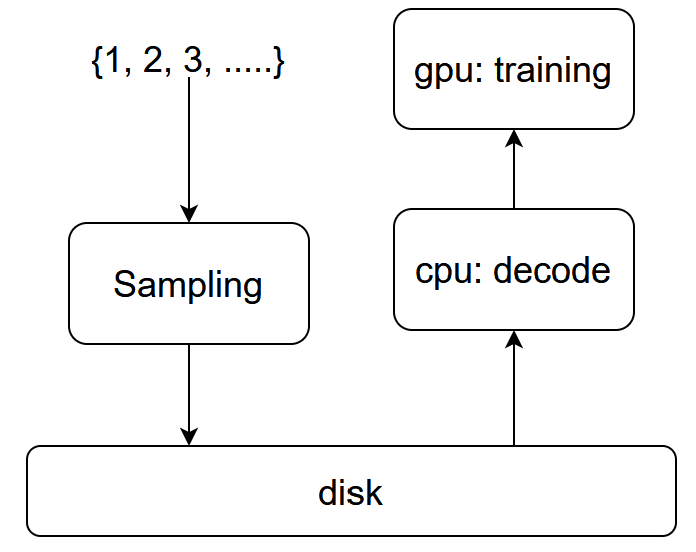
\includegraphics[height=4cm]{global_img_dir/data_pipeline.png}
    \end{center}
\end{frame}

\begin{frame}
    \frametitle{Problem}
    \begin{block}{Problem}
        The data will be repeatedly read and processed by different tasks.
    \end{block}
    \begin{block}{Configuration}
        Multiple tasks with worker = 4, batch size = 32 \\
        GPU: Tesla T4 with 16G memory, CPU: 48 Intel(R) Xeon(R) Gold 5118\\
    \end{block}
    \begin{figure}[htbp]
    \centering
    \begin{minipage}[t]{0.48\textwidth}
    \centering
    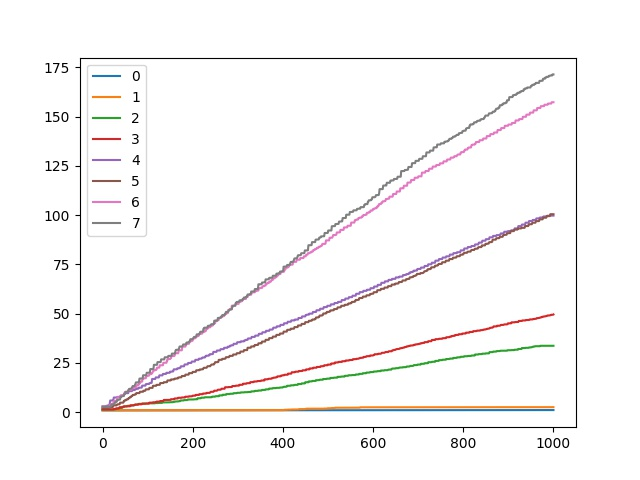
\includegraphics[width=5cm]{global_img_dir/l.jpg}
    \caption{data loading time}
    \end{minipage}
    \begin{minipage}[t]{0.48\textwidth}
    \centering
    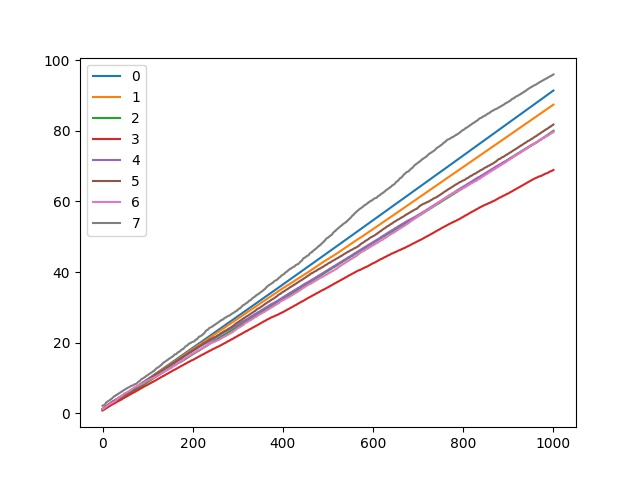
\includegraphics[width=5cm]{global_img_dir/b.jpg}
    \caption{data training time}
    \end{minipage}
    \end{figure}
\end{frame}

\begin{frame}
    \frametitle{Optimization}
    \begin{block}{Global Buffer Pool}
        \begin{itemize}
            \item If data in buffer pool, there is no need to read data from disk
        \end{itemize}
    \end{block}
    \centering
    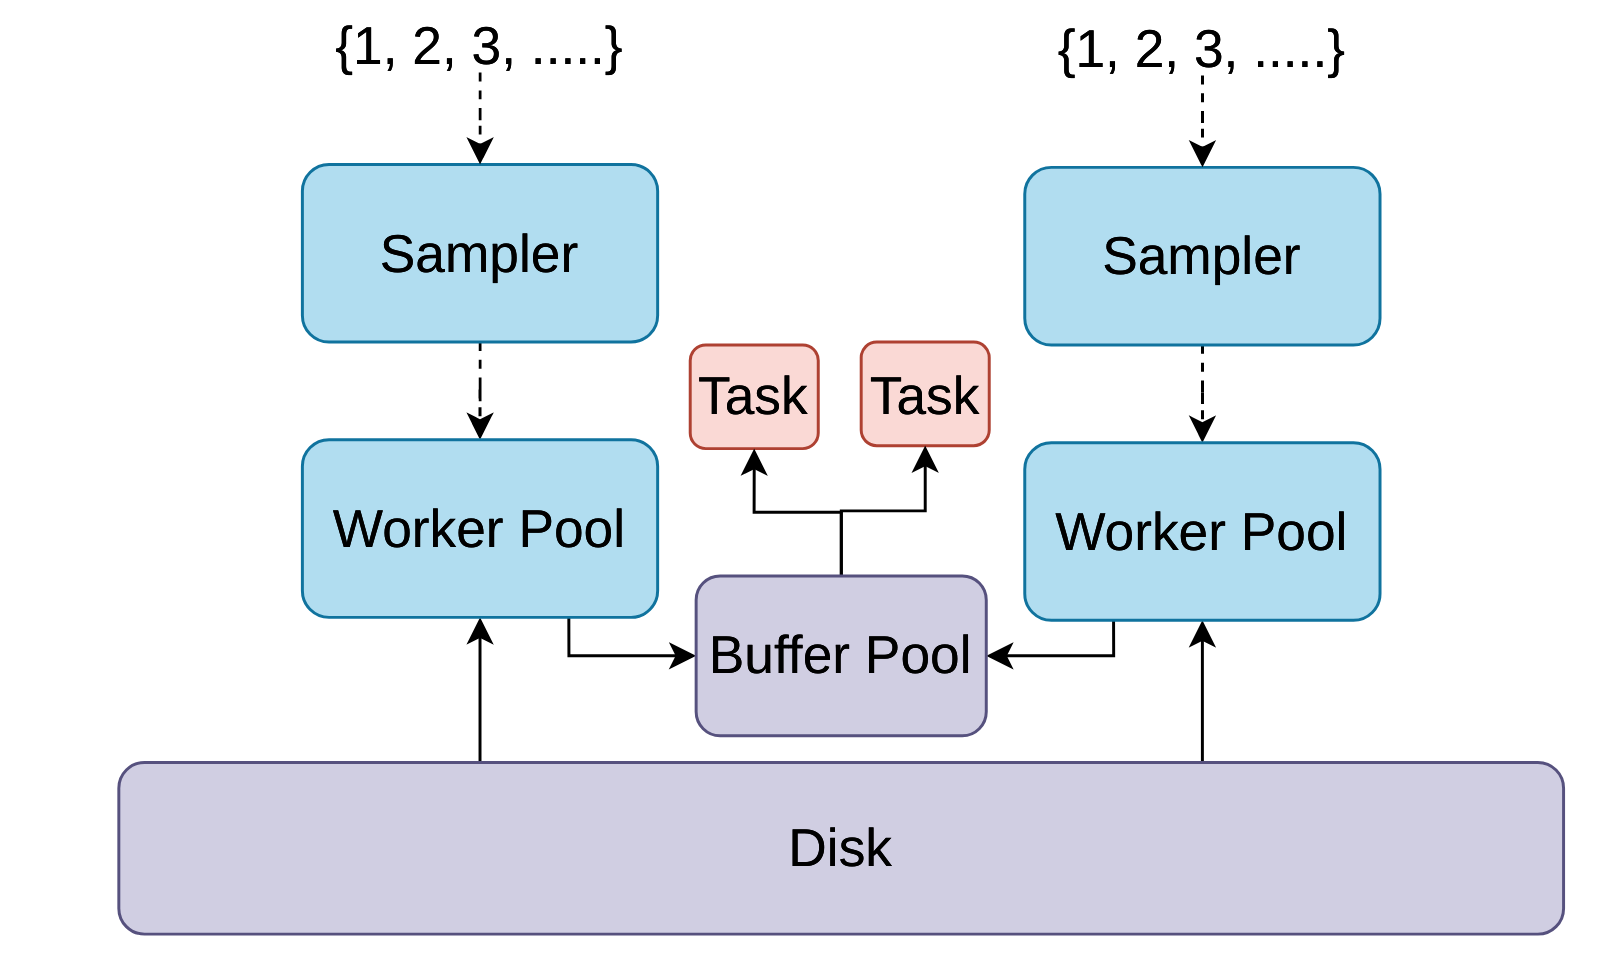
\includegraphics[width=8cm]{global_img_dir/global_buffer.png}
\end{frame}

\begin{frame}
    \frametitle{Problem}
    \begin{columns}
        \begin{column}{0.48\textwidth}
            \begin{itemize}
                \item Random replacement algorithm
            \end{itemize}
        \end{column}
        
        \begin{column}{0.48\textwidth}
            \begin{figure}
                \centering
                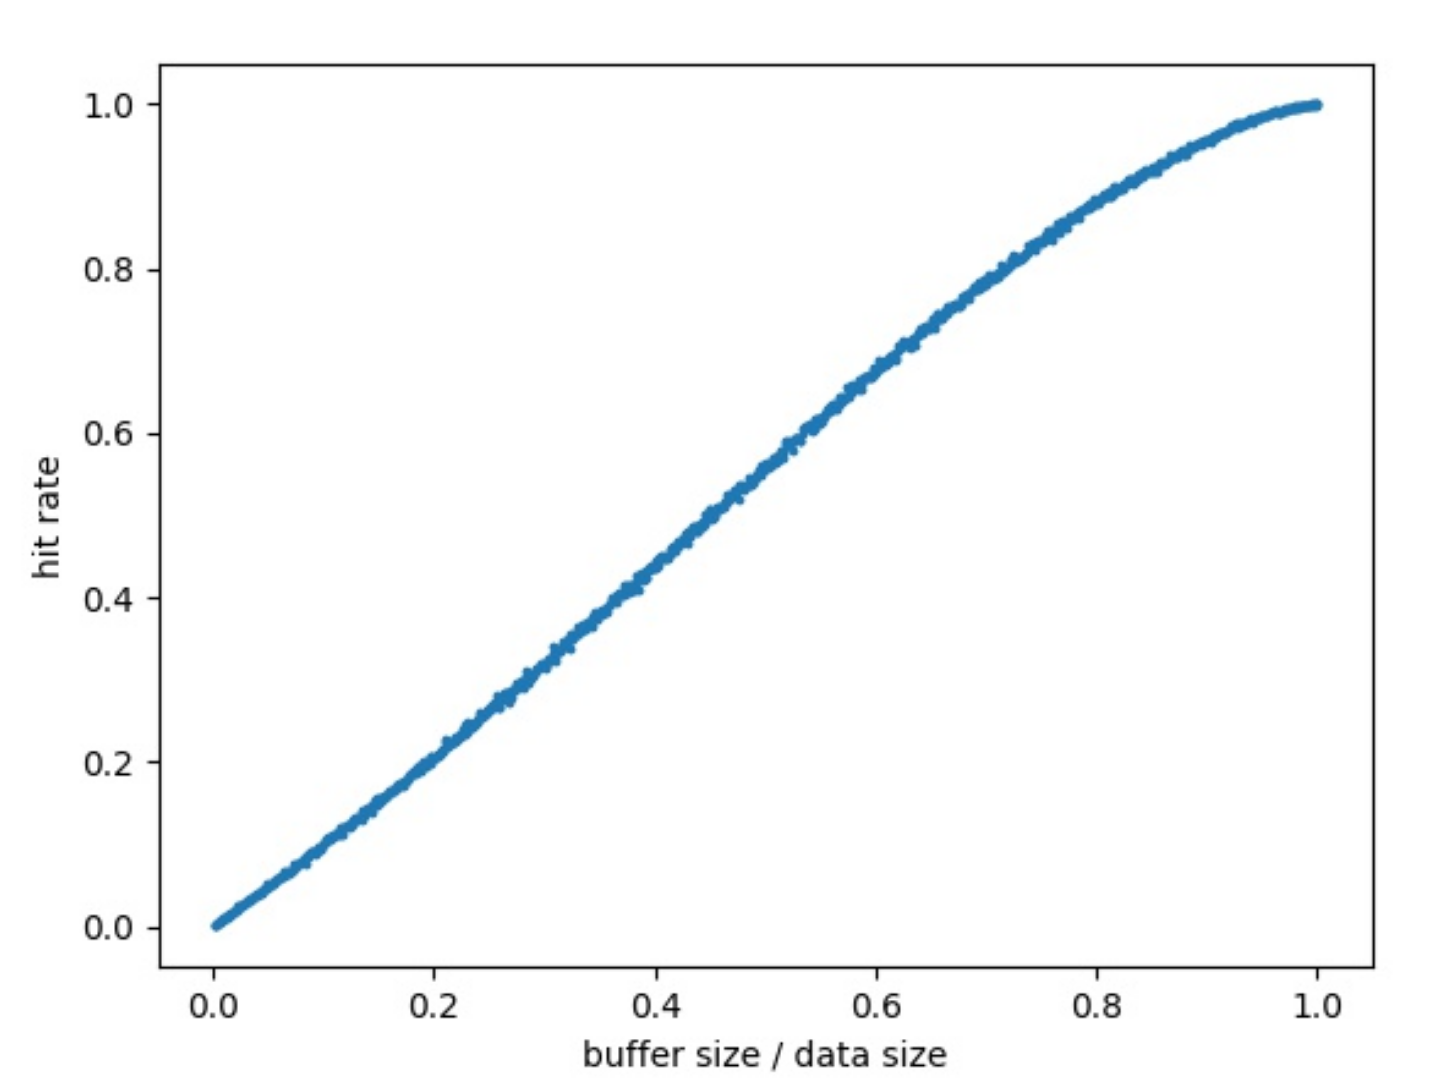
\includegraphics[width=6cm]{global_img_dir/random_hit_rate.png}
                \caption{hit rate with buffer size}
            \end{figure}
        \end{column}
    
    \end{columns}
\end{frame}

\begin{frame}
    \frametitle{Optimization}
    \begin{block}{Global Sampler}
        \begin{itemize}
            \item Make the sampled elements have a greater probability of being equal
        \end{itemize}
    \end{block}
    \centering
    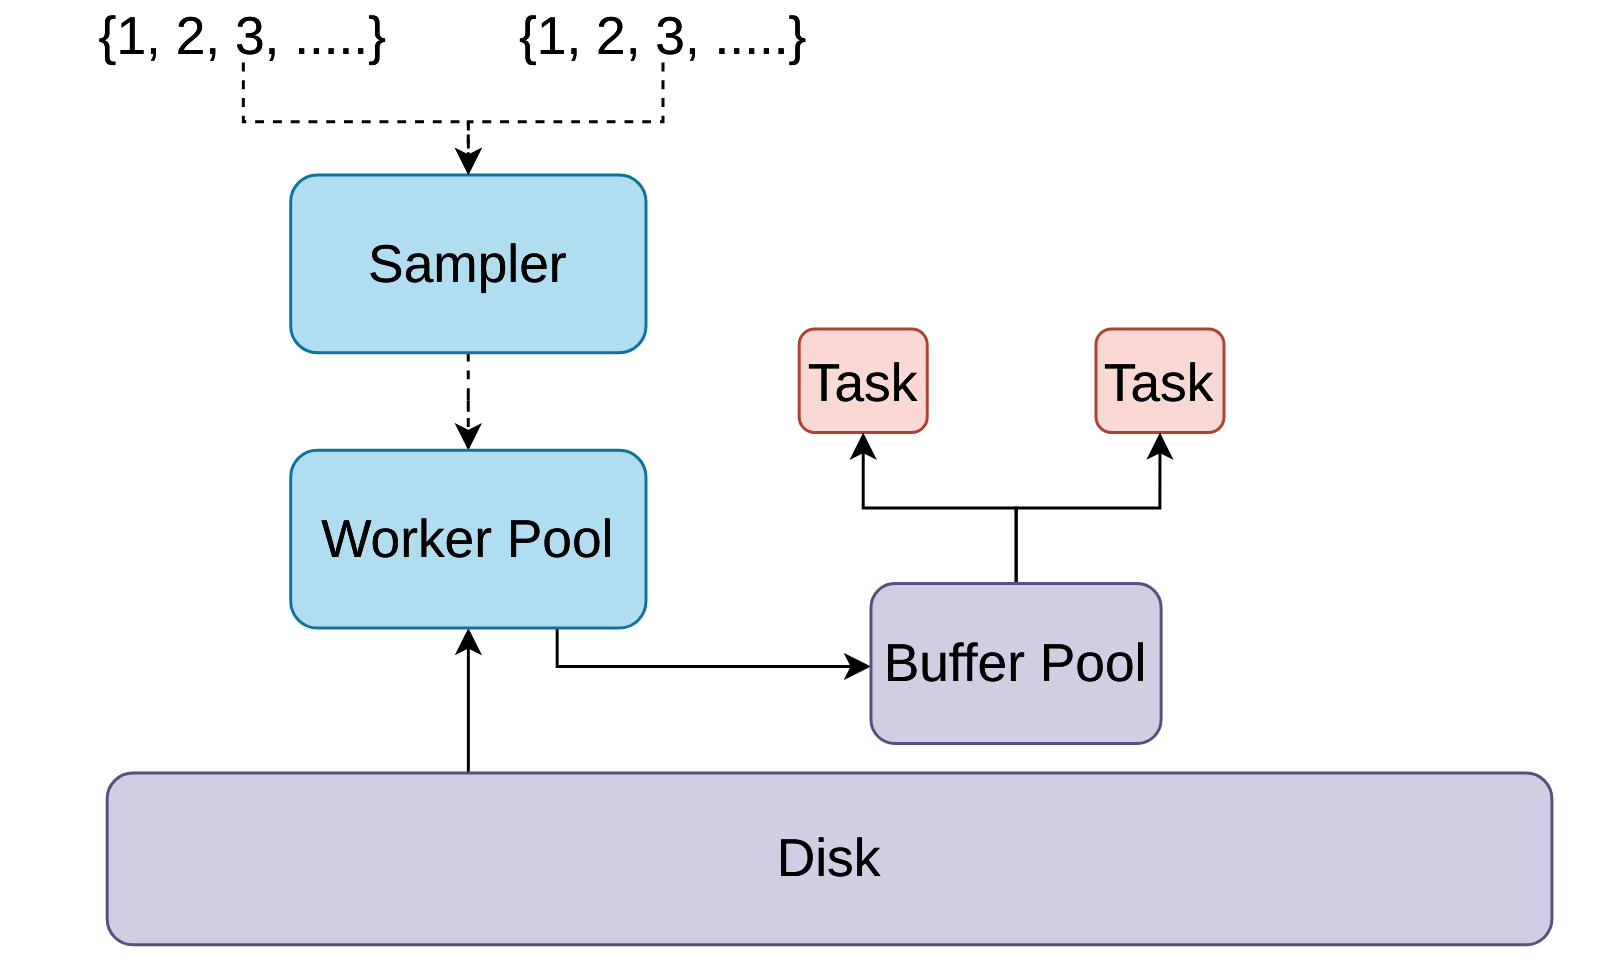
\includegraphics[width=8cm]{global_img_dir/global_sampling2.png}
\end{frame}


\section{Sampling Alogrithm}
\begin{frame}
    \frametitle{Sampling: problem description}
    \begin{block}{Defination}
        Assume there are two sets $\{S_1, S_2\}$, we should randomly select 2 elements $\{e_1, e_2\}$ from them.
        The algorithm should to make sure to:
        \begin{equation}
            \begin{aligned}
                & p(e_1) = \frac{1}{|S_1|}\\
                & p(e_2) = \frac{1}{|S_2|}\\
                & Maximize ( { p(e_1 = e_2) } )
            \end{aligned}
            \end{equation}
    \end{block}
    
\end{frame}

\begin{frame}
    \frametitle{Independently Sampling Algorithm}
    \begin{block}{Assumption}
        There are two sets: $S_1, S_2$, and their length is $n_1, n_2$ \\
        The intersection set of them is $S_i$, whose length is $n_i$ \\
        We divide the set $S_1$ into $S_i$ and $S_{d1} = S_1 - S_i$ \\
        We divide the set $S_2$ into $S_i$ and $S_{d2} = S_2 - S_i$ \\
        Sample(S): randomly select an element in S
    \end{block}
    
    \begin{block}{Example}
        $S_1 = \{1,2,3,4,5\} = \{1,2,3\} \cup \{4,5\}$ \\
        $S_2 = \{1,2,3,6,7\} = \{1,2,3\} \cup \{6,7\}$
    \end{block}
    
\end{frame}

\begin{frame}
    \frametitle{Independently Sampling Algorithm}
    \begin{columns}
        \begin{column}{0.48\textwidth}
            \begin{alertblock}{S1}
                \begin{itemize}
                    \item $step_{11}$:randomly select a set from $S_i$ and $S_{d1}$
                    \item $step_{21}$:if $S_{d1}$, $e_1$=Sample($S_{d1}$)
                    \item $step_{31}$:if $S_i$, $e_1$=Sample($S_{i}$)
                \end{itemize}
            \end{alertblock}
        \end{column}
        
        \begin{column}{0.48\textwidth}
        \begin{alertblock}{S2}
            \begin{itemize}
                \item $step_{12}$:randomly select a set from $S_i$ and $S_{d2}$
                \item $step_{22}$:if $S_{d2}$, $e_2$=Sample($S_{d2}$)
                \item $step_{32}$:if $S_i$, $e_2$=Sample($S_{i}$)
            \end{itemize}
        \end{alertblock}
        \end{column}
    
    \end{columns}

    \begin{block}{Probability}
    \begin{equation}
        \begin{aligned}
            p(e_1 = e_2) = \frac{n_i}{n_1*n_2}
        \end{aligned}
    \end{equation}
    \end{block}
\end{frame}

% \begin{frame}
%     \frametitle{Independently Sampling Algorithm}
%     % \begin{block}{Algorithm}
%         % \begin{itemize}
%             \begin{columns}
%             \begin{column}{0.5\textwidth}
%             % \item $S_1$:
%             fdfd
%             % \begin{itemize}
%             %     \item $step_{11}$: randomly select a set from $S_i$ and $S_{d1}$
%             %     \item $step_{12}$: if the set is $S_{d1}$, randomly select a element $e_1$ from $S_{d1}$
%             %     \item $step_{13}$: if the set is $S_i$, randomly select a element $e_1$ from $S_i$
%             % \end{itemize}
%             \end{column}
%             \begin{column}{0.5\textwidth}
%                 dsdsds
%             % \item $S_2$:
%             % \begin{itemize}
%             %     \item $step_{21}$: randomly select a set from $S_i$ and $S_{d2}$
%             %     \item $step_{22}$: if the set is $S_{d2}$, randomly select a element $e_2$ from $S_{d2}$
%             %     \item $step_{23}$: if the set is $S_i$, randomly select a element $e_2$ from $S_i$
%             % \end{itemize}
%             \end{column}
%             \end{columns}
%         % \end{itemize}
%     \end{block}
%     \begin{block}{Probability}
%         \begin{equation}
%             \begin{aligned}
%                 p(e_1) = \frac{1}{n_1},p(e_2) = \frac{1}{n_2}\\
%                 p(e_1 = e_2) = \frac{n_i}{n_1*n_2}
%             \end{aligned}
%         \end{equation}
%     \end{block}
% \end{frame}

\begin{frame}
    \frametitle{Dependently Sampling Algorithm I}
    \begin{block}{Insight}
        The $step_{31}$ is same as $step_{32}$ (randomly select an element $e$ from $S_i$).
    \end{block}
    \begin{block}{Example}
        $S_1 =  \{1,2,3\} \cup \{4,5\}$; $S_2 = \{1,2,3\} \cup \{6,7\}$
        \begin{itemize}
            \item Firstly, randomly sampling element $e_i$ in $\{1,2,3\}$
            \item As for $S_1$, if select set $\{1,2,3\}$ with probability $p_1(S_i)=0.6$, then we can let $e_1 = e_i$
            \item As for $S_2$, select set $\{1,2,3\}$ with probability $p_2(S_i)=0.6$, then we can let $e_2 = e_i$
            \item $p(e_1 = e_2) = p_1(S_i)*p_2(S_i) = 0.36$
        \end{itemize}
    \end{block}
\end{frame}

\begin{frame}
    \frametitle{Dependently Sampling Algorithm I}
    \begin{block}{Algorithm}
        \begin{itemize}
            \item $step_{0}$: $e_i$ = Sample($S_i$)
        \end{itemize}
        \begin{columns}
        \begin{column}{0.5\textwidth}
            \begin{alertblock}{S1}
                \begin{itemize}
                    \item $step_{11}$:randomly select a set from $S_i$ and $S_{d1}$
                    \item $step_{21}$:if $S_{d1}$,$e_1$ = Sample($S_{d1}$)
                    \item $step_{31}$:if $S_i$, $e_1$ = $e_i$
                \end{itemize}
            \end{alertblock}
            \end{column}
            \begin{column}{0.5\textwidth}
            \begin{alertblock}{S2}
                \begin{itemize}
                    \item $step_{12}$:randomly select a set from $S_i$ and $S_{d2}$
                    \item $step_{22}$:if $S_{d2}$, $e_2$ = Sample($S_{d2}$)
                    \item $step_{32}$:if $S_i$, $e_2$ = $e_i$
                \end{itemize}
            \end{alertblock}
            \end{column}
        \end{columns}
    \end{block}

    \begin{block}{Probability}
        \begin{equation}
            \begin{aligned}
                p(e_1 = e_2) &=  \frac{n_i}{n_1}*\frac{n_i}{n_2} = \frac{n_i^2}{n_1*n_2}
            \end{aligned}
        \end{equation}
    \end{block}
\end{frame}

\begin{frame}
    \frametitle{Dependently Sampling Algorithm I}
    \begin{block}{Insight}
        The $step_{11}$ and $step_{12}$ are similar. We can merge them.
    \end{block}
    \begin{block}{Example}
        $S_1 =  \{1,2,3\} \cup \{4,5\}$; $S_2 = \{1,2,3\} \cup \{6,7\}$
        \begin{itemize}
            \item Firstly, we randomly select a set from $\{1,2,3\}$ and $\{4,5\}$
            \item If we choose $\{1,2,3\}$, the S1 and S2 will both select an element from $\{1,2,3\}$
            \item If we choose $\{4,5\}$, then S1 will sampling in $\{4,5\}$ and S2 in $\{6,7\}$
            \item $p(e_1 = e_2) = p_1(S_i) = 0.6$
        \end{itemize}
    \end{block}
\end{frame}

\begin{frame}
    \frametitle{Dependently Sampling Algorithm II}
    \begin{block}{Algorithm}
        \begin{itemize}
            \item $step_{0}$: $e_i$ = Sample($S_i$)
            \item $step_{1}$: randomly select a set from $S_i$ and $S_{d1}$
            \begin{columns}
                \begin{column}{0.48\textwidth}
                    \begin{alertblock}{S1}
                        \begin{itemize}
                            \item $step_{21}$: if $S_{d1}$,$e_1$=Sample($S_{d1}$)
                            \item $step_{31}$: if $S_i$, $e_1=e_i$
                        \end{itemize}
                    \end{alertblock}
                    \end{column}
                    \begin{column}{0.48\textwidth}
                    \begin{alertblock}{S2}
                        \begin{itemize}
                            \item $step_{22}$: if $S_{d1}$,$e_2$=Sample($S_{d2}$)
                            \item $step_{32}$: if $S_i$, $e_2=e_i$
                        \end{itemize}
                    \end{alertblock}
                \end{column}
            \end{columns}
        \end{itemize}
    \end{block}
\end{frame}

\begin{frame}
    \frametitle{Problem:$n_1 \neq n_2$}
    \begin{block}{$n_1 > n_2$}
        $S_1 =  \{1,2,3\} \cup \{4\}$; $S_2 = \{1,2,3\} \cup \{6,7\}$
        \begin{itemize}
            \item $S_1$ select $\{1,2,3\}$ with probability $p_1(S_i) = 0.75$
            \item Then $S_2$ select an element $e$ from $S_i$ with probability $p_2(e) = p_1(S_i)*\frac{1}{3} = 0.25 > 0.2$
        \end{itemize}
    \end{block}
    \begin{block}{$n_1 < n_2$}
        $S_1 =  \{1,2,3\} \cup \{4,6\}$; $S_2 = \{1,2,3\} \cup \{7\}$
        \begin{itemize}
            \item $S_1$ select $\{4,6\}$ with probability $p_1(S_{d1}) = 0.4$
            \item Then $S_2$ select an element $e$ from $S_{d2}$ with probability $p_2(e) = p_1(S_{d1})*\frac{1}{1} = 0.4 > 0.25$
        \end{itemize}
    \end{block}
\end{frame}

\begin{frame}
    \frametitle{Case1: n1 < n2}
    \begin{block}{Problem}
        \begin{equation}
            \begin{aligned}
                (p_1(S_i) = \frac{n_i}{n_1}) > (p_2(S_i) = \frac{n_i}{n_2}) \\
            \end{aligned}
        \end{equation}
    \end{block}
    \begin{block}{Approach}
        So in $step_1$, when select $S_i$, it should be changed $S_{d2}$ in probability of $p$. \\
        \begin{equation}
            \left\{
            \begin{aligned}
                    p_2(S_i) &= p_1(S_i)*(1-p) = \frac{n_i}{n_2} \\
                    p_2(S_{d2}) &= p_2(S_{d1})+p_1(S_i)*{p} = 1-\frac{n_i}{n_2} \\
            \end{aligned}
            \right. 
        \end{equation}
        \begin{equation}
            p = 1-\frac{n_1}{n_2}
        \end{equation}
    \end{block}
\end{frame}

\begin{frame}
    \frametitle{Dependently Sampling Algorithm II}
    \begin{block}{Algorithm}
        \begin{itemize}
            \item $step_{0}$: $e_i$ = Sample($S_i$)
            \item $step_{1}$: randomly select a set from $S_i$ and $S_{d1}$
            \begin{columns}
                \begin{column}{0.48\textwidth}
                    \begin{alertblock}{S1}
                        \begin{itemize}
                            \item $step_{21}$:if $S_{d1}$, $e_1$=Sample($S_{d1}$)
                            \item $step_{31}$:if $S_i$, $e_1 = e_i$
                        \end{itemize}
                    \end{alertblock}
                    \end{column}
                    \begin{column}{0.48\textwidth}
                    \begin{alertblock}{S2}
                        \begin{itemize}
                            \item $step_{22}$: if $S_{d1}$, $e_2$=Sample($S_{d2}$)
                            \item $step_{32}$: if $S_i$:
                            \begin{itemize}
                                \item let $S = S_{d1}$ in probability of $1-\frac{n_1}{n_2}$
                                \item if $S_{d1}$, $e_2$=Sample($S_{d2}$)
                                \item if $S_i$, $e_2 = e_i$
                            \end{itemize}
                        \end{itemize}
                    \end{alertblock}
                \end{column}
            \end{columns}
        \end{itemize}
    \end{block}
    
    \begin{block}{Probability}
        % If in $step_1$, the selected set $S = S_i$, and $p_1(S_i) = \frac{n_i}{n_1}$
        % $$
        %     p(element2) = p_1(S_i)*(\frac{n_1}{n_2})*\frac{1}{n_i} = \frac{1}{n_2}
        % $$
        % If in $step_1$, the selected set $S = S_{d1}$, and $p_1(S_{d1}) = 1-\frac{n_i}{n_1}$
        % $$
        %     p(element2) = (p_1(S_{d1})+(1-\frac{n_1}{n_2})*p_1(S_i))*\frac{1}{n_2-n_i} = \frac{1}{n_2}
        % $$
        % and
        $$
            p(e_1 = e_2) = p_1(S_i)*(\frac{n_1}{n_2}) = \frac{n_i}{n_2}
        $$
    \end{block}
\end{frame}

\begin{frame}
    \frametitle{Case2: n1 > n2}
    \begin{block}{Problem}
        \begin{equation}
            \begin{aligned}
                (p_1(S_{d1}) = 1-\frac{n_i}{n_1}) > (p_2(S_{d_2}) = 1-\frac{n_i}{n_2}) \\
            \end{aligned}
        \end{equation}
    \end{block}
    \begin{block}{Approach}
        So in $step_1$, when select $S_{d1}$, it should be changed $S_{i}$ in probability of $p$. \\
        The equation is 
            \begin{equation}
                \left\{
                \begin{aligned}
                    p_2(S_i) &= p_1(S_i)+p_2(S_{d1})*p = \frac{n_i}{n_2} \\
                    p_2(S_{d2}) &= p_2(S_{d1})*(1-p) = 1-\frac{n_i}{n_2}
                \end{aligned}
                \right. 
            \end{equation}
            \begin{equation}
                p = 1-\frac{n1*(n2-n_i)}{n2*(n1-n_i)}
            \end{equation}
    \end{block}
\end{frame}

\begin{frame}
    \frametitle{Dependently Sampling Algorithm II}
    \begin{block}{Algorithm}

        \begin{itemize}
            \item $step_{0}$: $e_i$ = Sample($S_i$)
            \item $step_{1}$: randomly select a set from $S_i$ and $S_{d1}$
            \begin{columns}
                \begin{column}{0.48\textwidth}
                    \begin{alertblock}{S1}
                        \begin{itemize}
                            \item $step_{21}$:if $S_{d1}$, $e_1$=Sample($S_{d1}$)
                            \item $step_{31}$:if $S_i$, $e_1 = e_i$
                        \end{itemize}
                    \end{alertblock}
                    \end{column}
                    \begin{column}{0.48\textwidth}
                    \begin{alertblock}{S2}
                        \begin{itemize}
                            \item $step_{22}$: if $S_{d1}$:
                            \begin{itemize}
                                \item let $S = S_{i}$ in probability of $1-\frac{n1*(n2-n_i)}{n2*(n1-n_i)}$
                                \item if $S_{d1}$, $e_2$=Sample($S_{d2}$)
                                \item if $S_i$, $e_2 = e_i$
                            \end{itemize}
                            \item $step_{32}$: if $S_i$, $e_2 = e_i$
                        \end{itemize}
                    \end{alertblock}
                \end{column}
            \end{columns}
        \end{itemize}
    \end{block}
    \begin{block}{Probability}
        % If in $step_1$, the selected set $S = S_i$
        % $$
        %     p(element2) = (p_1(S_i)+p_2(S_{d1})*p)*\frac{1}{n_i} = \frac{1}{n_2}
        % $$
        % If in $step_1$, the selected set $S = S_{d1}$, and $p_1(S_{d1}) = 1-\frac{n_i}{n_1}$
        % $$
        %     p(element2) = ( p_2(S_{d1})*(1-p))*\frac{1}{n_2-n_i} = \frac{1}{n_2}
        % $$
        % and
        $$
            p(e_1 = e_2) = p_1(S_i) = \frac{n_i}{n_1}
        $$
    \end{block}
\end{frame}

\begin{frame}
    \frametitle{Why not shuffle $S_1 \cup S_2$}
    \begin{block} {Probability}
        $p(e_1=e_2) = \frac{|S_1\cap S_2|}{|S_1 \cup S_2|} < \frac{|S_1\cap S_2|}{max(|S_1|,|S_2|)}$
    \end{block}
    \begin{block} {randomly select in $S_1\cup S_2$: "starvation"}
        if $|S_1| = 99, |S_2| = 1$,
        then $p(e \in S_1) = 0.99, p(e \in S_2) = 0.01$ \\
        So task2 may be starving
    \end{block}
    \begin{block} {shuffle $S_1\cup S_2$: offset}
        $S_1 = \{2,3\}, S_2 = \{1,2,3\}$\\
        \{\space \space  2,3\}\\
        \{1,2,3\} \\
        \{1,2,3\}\\
    \end{block}
\end{frame}


\begin{frame}
    \frametitle{Sampling Tree: there are two sets: $S_1, S_2$}
    \begin{columns}
        \begin{column}{0.48\textwidth}
            \begin{itemize}
                \item $A = S_1\cap S_2$
                \item $B = S_1- A$
                \item $A = S_2\cap A$
            \end{itemize}
        \end{column}
        \begin{column}{0.48\textwidth}
            \begin{figure}
                \centering
                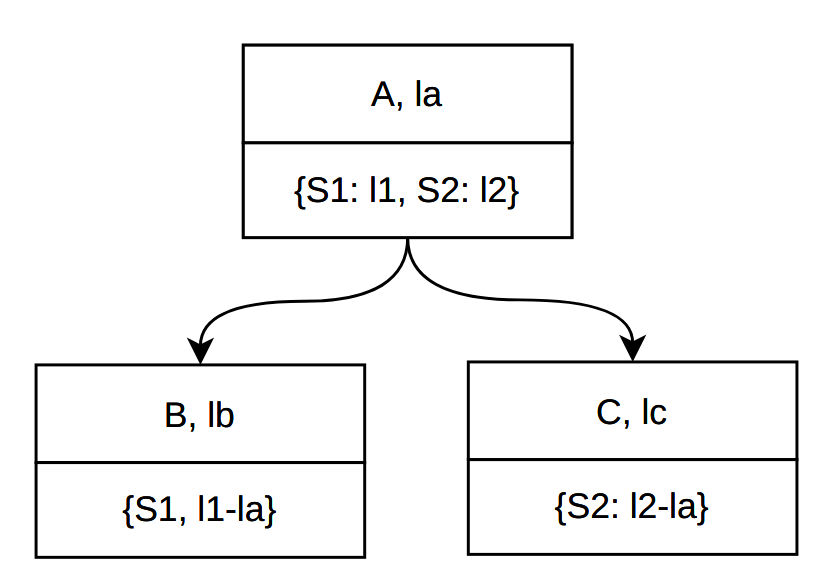
\includegraphics[width=6cm]{global_img_dir/st1.png}
                \caption{Sampling Tree}
            \end{figure}
        \end{column}
    \end{columns}
\end{frame}

\begin{frame}
    \frametitle{Sampling Tree: insert $S_3$}
    \begin{columns}
        \begin{column}{0.48\textwidth}
            \begin{itemize}
                \item $A \subset S_3$
                \item Insert $\{S_3: l_3\}$ in $A$ ascending order
                \item $S_3 = S_3 - A$
                \item Insert $S_3$ in subtree that has the largest intersection with $S_3$
            \end{itemize}
        \end{column}
        \begin{column}{0.48\textwidth}
            \begin{figure}
                \centering
                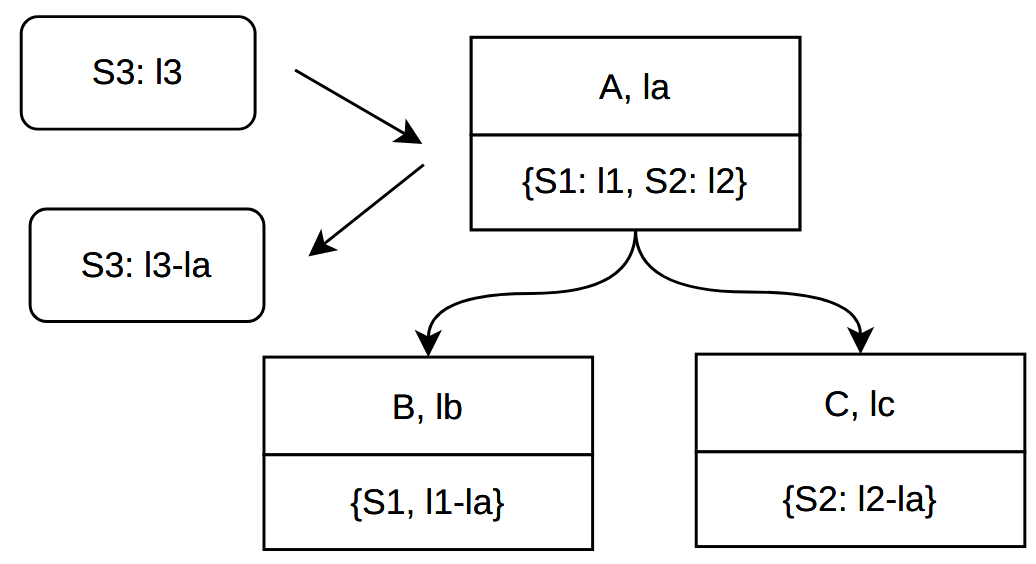
\includegraphics[width=6cm]{global_img_dir/insert1.png}
                \caption{Sampling Tree}
            \end{figure}
        \end{column}
    \end{columns}
\end{frame}

\begin{frame}
    \frametitle{Sampling Tree: Insert $S_3$}
    \begin{columns}
        \begin{column}{0.48\textwidth}
            \begin{itemize}
                \item $B \not\subset S_3$
                \item Create new node: $D = S_3 \cap B$
                \item $E = B-D$
                \item $F = S_3-D$
            \end{itemize}
        \end{column}
        \begin{column}{0.48\textwidth}
            \begin{figure}
                \centering
                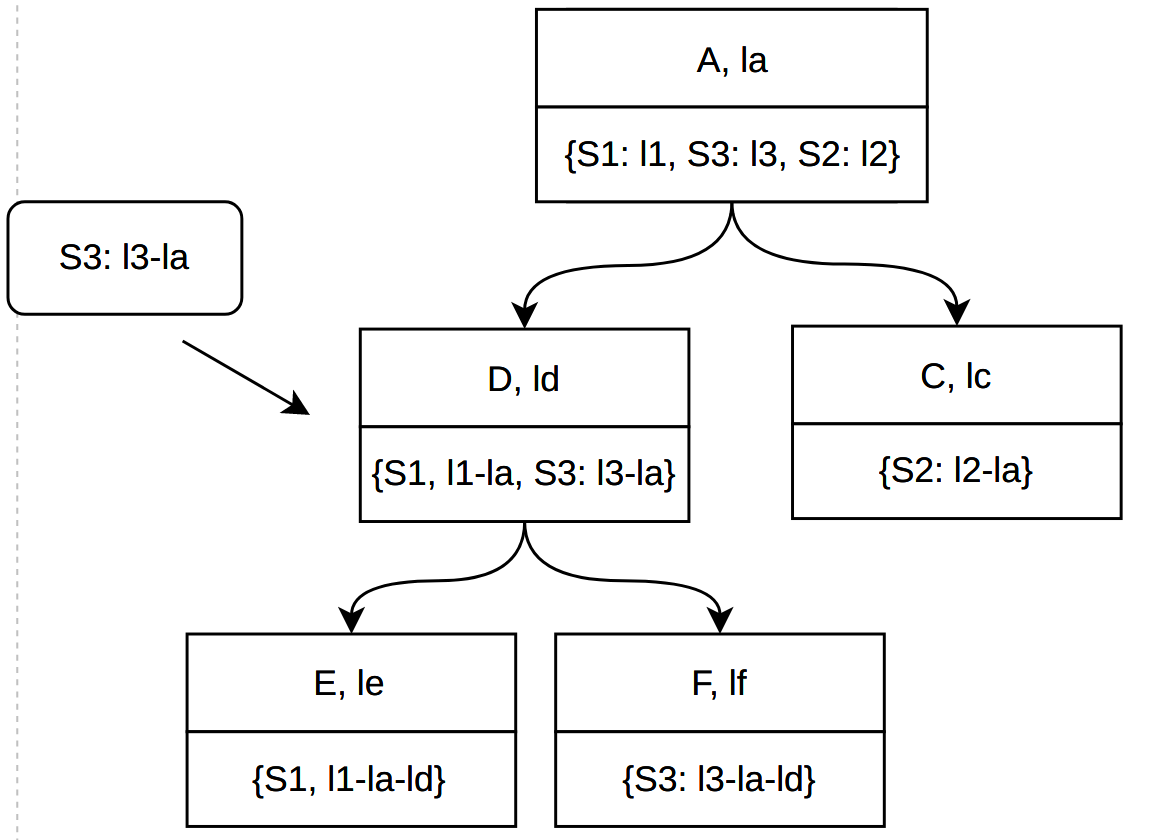
\includegraphics[width=6cm]{global_img_dir/insert2.png}
                \caption{Sampling Tree}
            \end{figure}
        \end{column}
    \end{columns}
\end{frame}

\begin{frame}
    \frametitle{Sampling Tree: Delete $S_3$}
    \begin{columns}
        \begin{column}{0.48\textwidth}
            \begin{itemize}
                \item Delete $S_3$ in root
                \item Recursively let the subtree delete $S_3$
                \item Until reaching the leaf node, then delete it
                \item The corresponding parent node merges the child nodes
            \end{itemize}
        \end{column}
        \begin{column}{0.48\textwidth}
            \begin{figure}
                \centering
                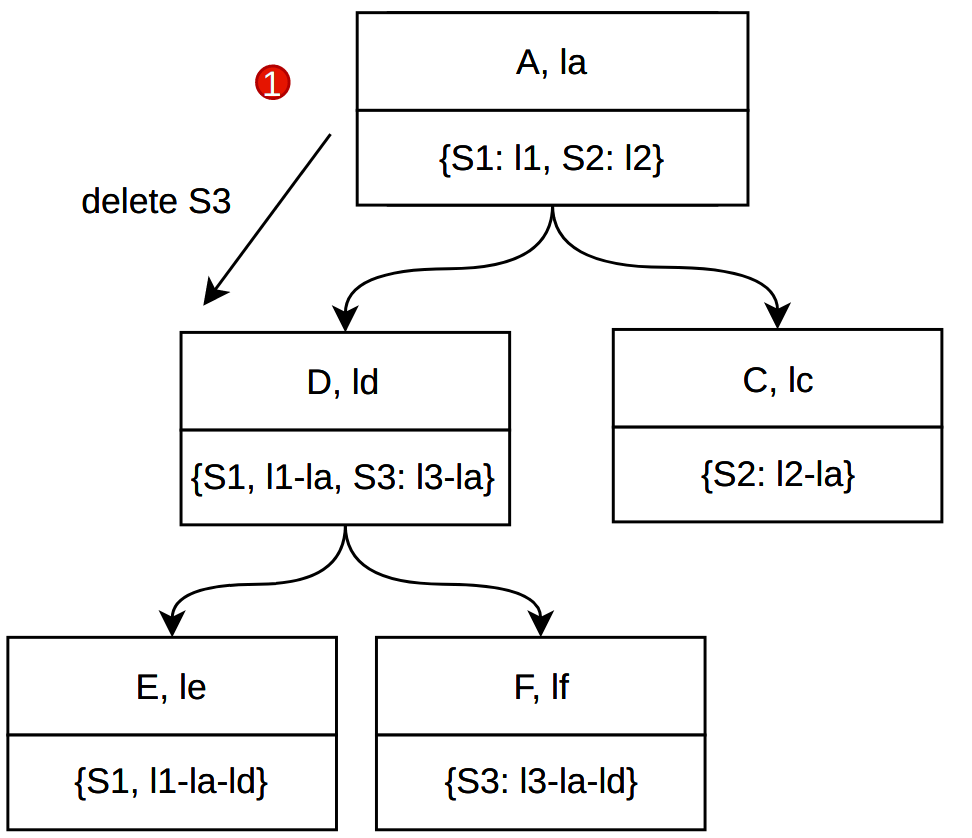
\includegraphics[width=6cm]{global_img_dir/delete1.png}
                \caption{Sampling Tree}
            \end{figure}
        \end{column}
    \end{columns}
\end{frame}

\begin{frame}
    \frametitle{Sampling Tree: Sampling in root}
    \begin{columns}
        \begin{column}{0.48\textwidth}
            \begin{itemize}
                \item Split U into $parent$ and $child$
                \begin{itemize}
                    \item $p < \frac{l_a}{l_1}, parent \cup \{S1\}$
                    \item ......
                    \item $p > \frac{l_i}{l_{i+1}}, child \cup \{S_i, S_{i+1}, ... \}$
                \end{itemize}
                \item Sampling e in A, which represents the sampling result of $parent$
                \item Push down $child$
                \item Because $e \notin A$, so we need to push down $e$ and the collection $U_e$ containing it
            \end{itemize}
        \end{column}
        \begin{column}{0.48\textwidth}
            \begin{figure}
                \centering
                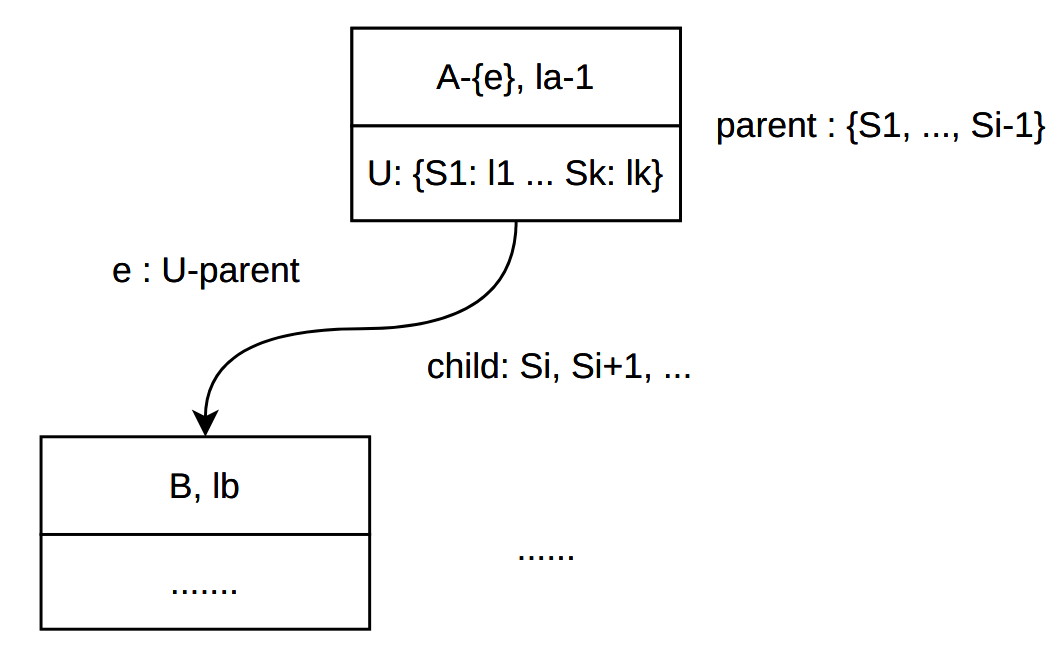
\includegraphics[width=6cm]{global_img_dir/sp1.png}
                \caption{Sampling Tree}
            \end{figure}
        \end{column}
    \end{columns}
\end{frame}

\begin{frame}
    \frametitle{Sampling Tree: Sampling in child}
    \begin{columns}
        \begin{column}{0.48\textwidth}
            \begin{itemize}
                \item Split child into $parent$ and $child$
                \item Sampling e in A, which represents the sampling result of $parent$
                \item Push down $child$
                \item Because $e \notin A$, so we need to push down $e$ and the collection containing it
                \item if $U_e \subset U$, then add e in this node
            \end{itemize}
        \end{column}
        \begin{column}{0.48\textwidth}
            \begin{figure}
                \centering
                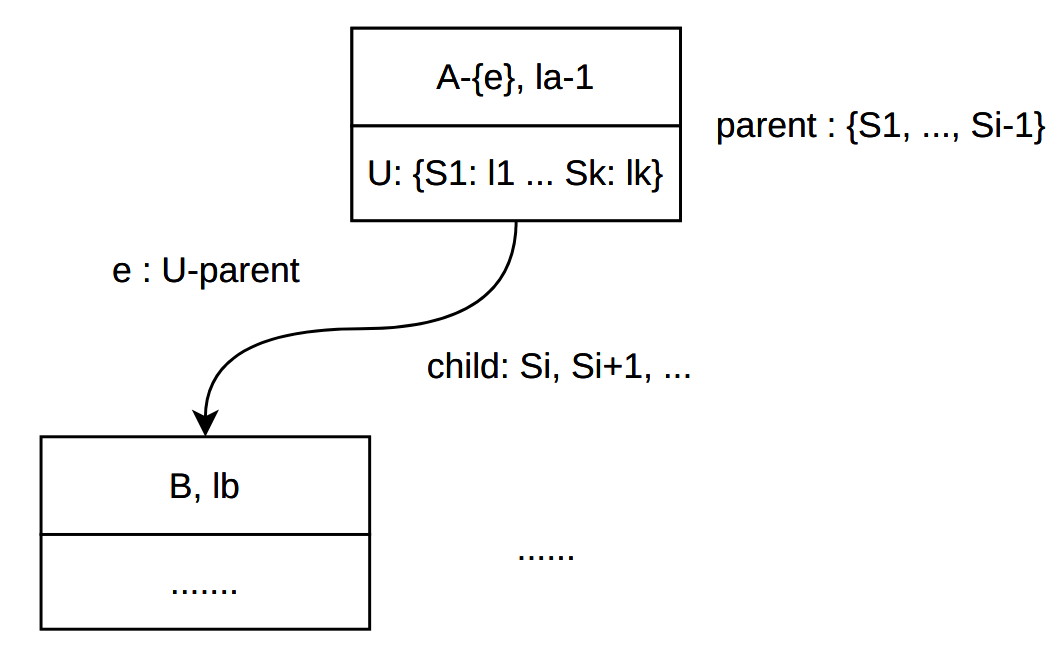
\includegraphics[width=6cm]{global_img_dir/sp1.png}
                \caption{Sampling Tree}
            \end{figure}
        \end{column}
    \end{columns}
\end{frame}

\begin{frame}
    \frametitle{Example}
    \centering
    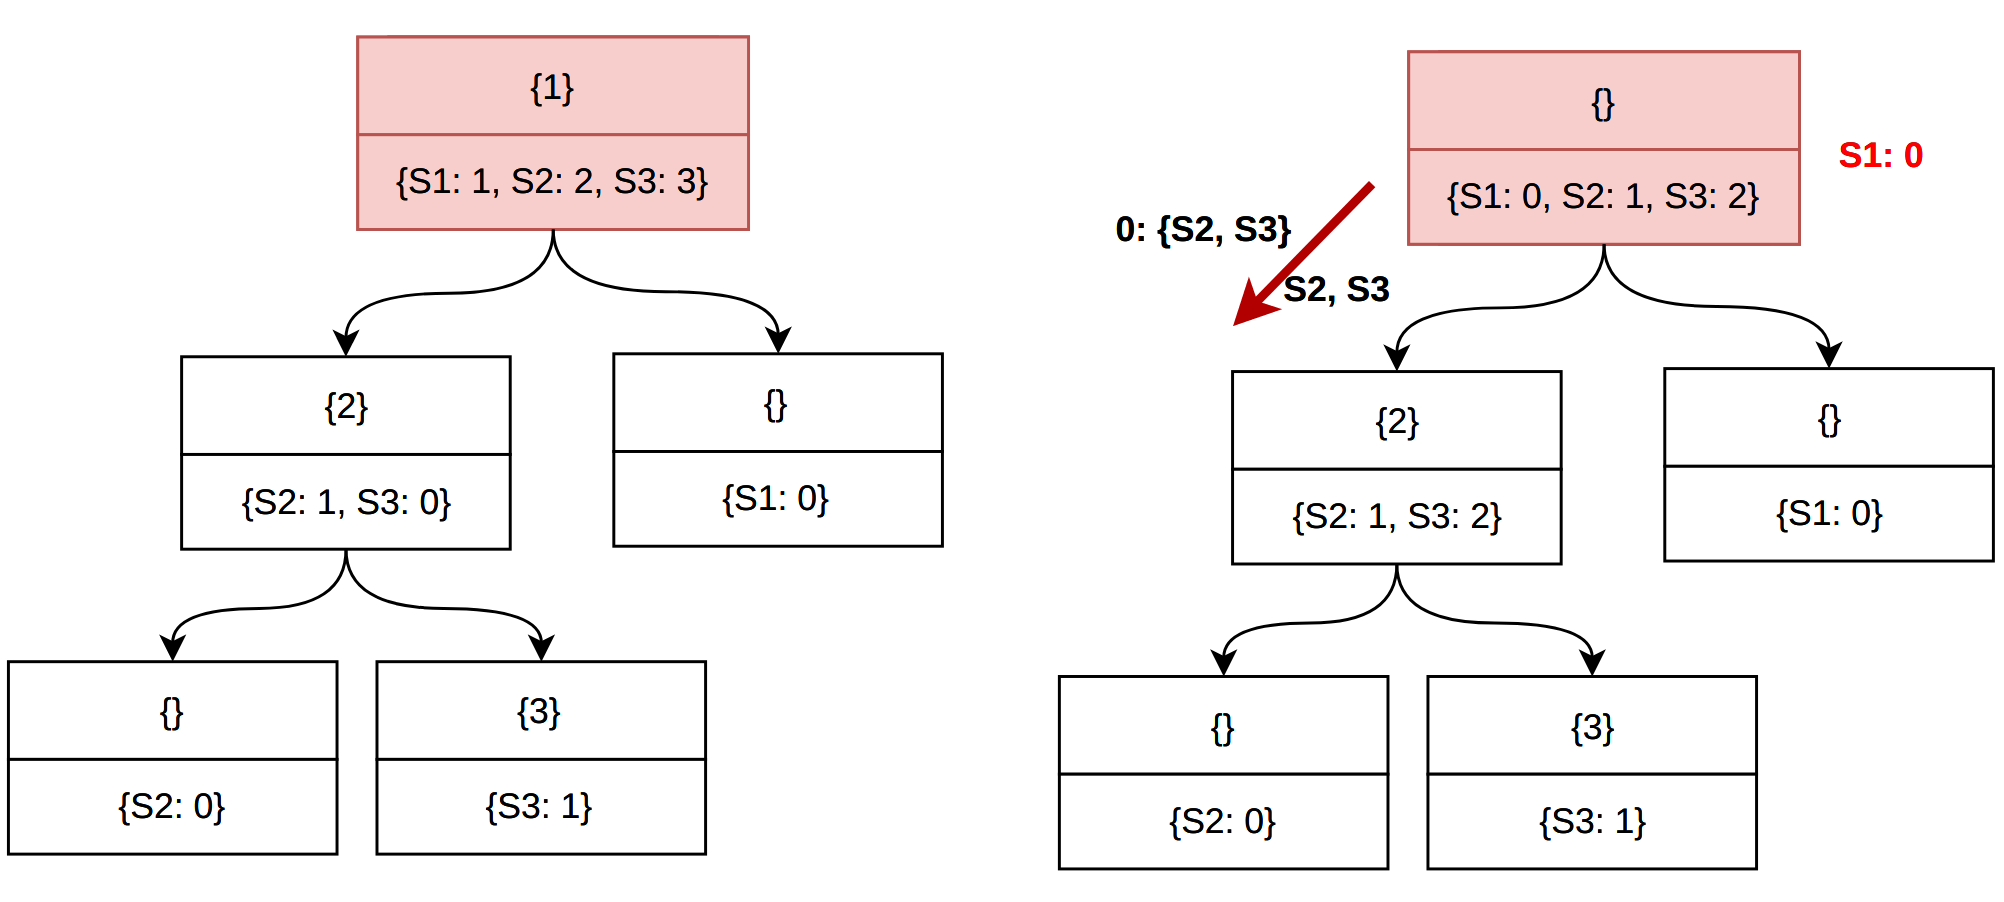
\includegraphics[width=12cm]{global_img_dir/exa1.png}
\end{frame}

\begin{frame}
    \frametitle{Example}
    \centering
    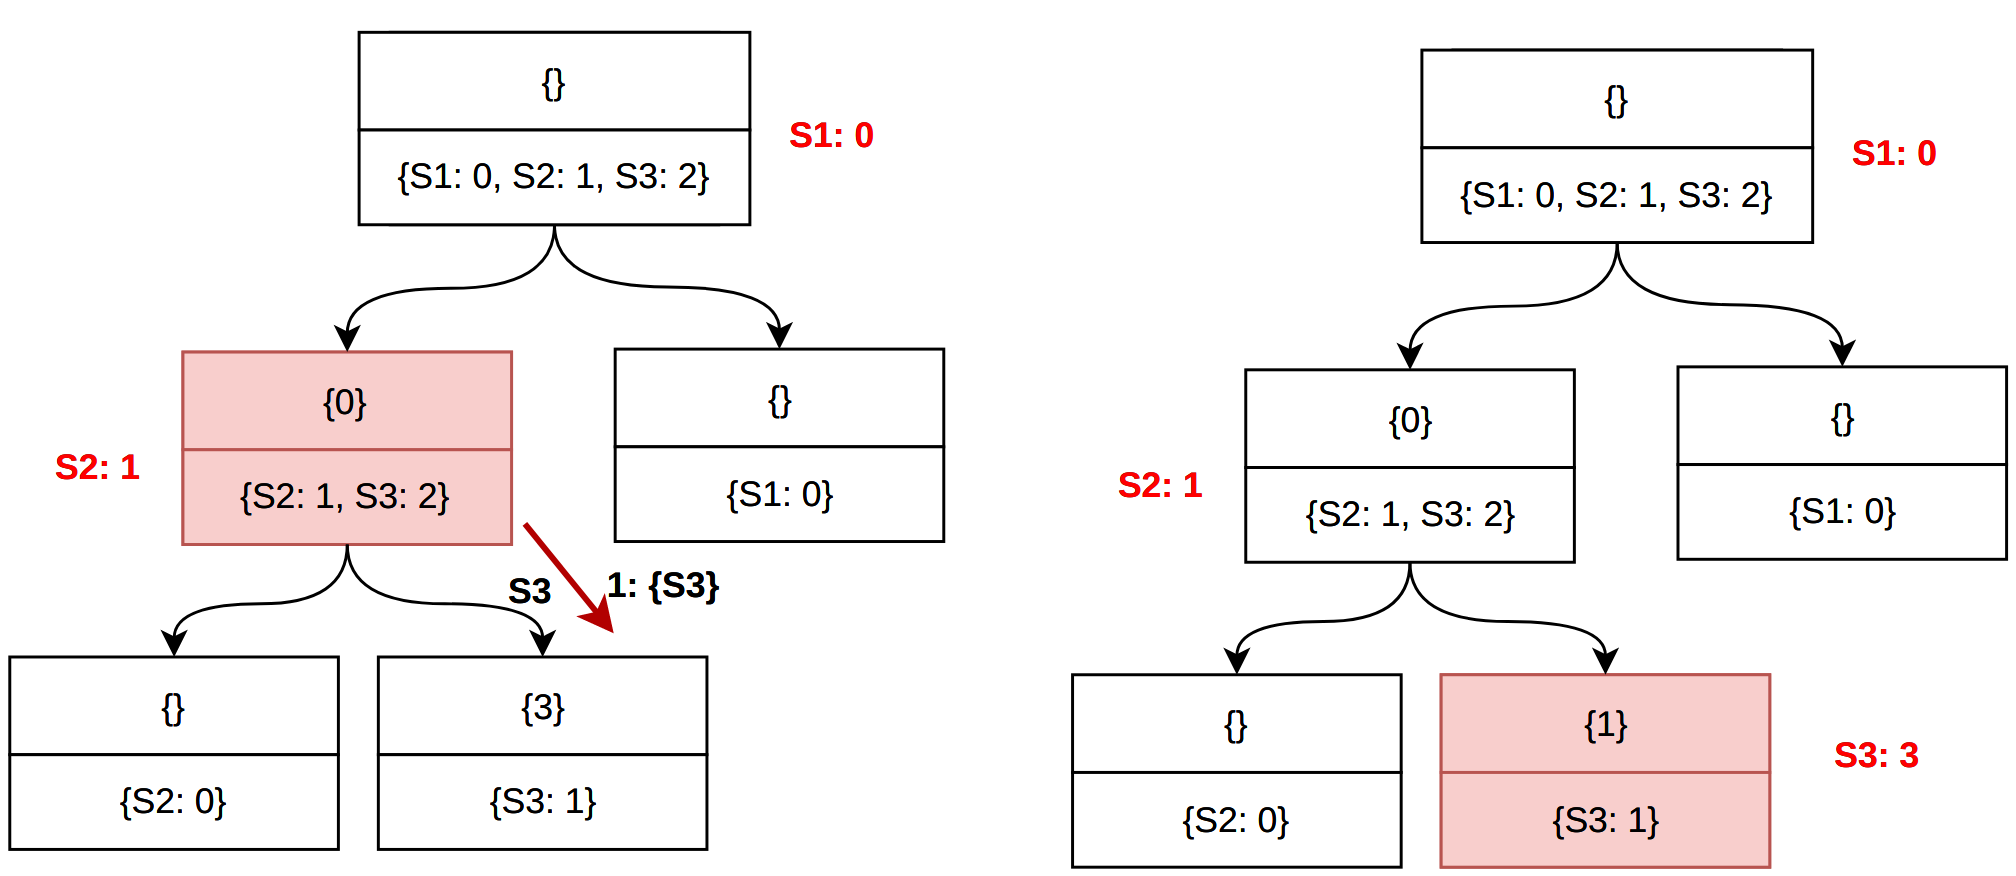
\includegraphics[width=12cm]{global_img_dir/exp2.png}
\end{frame}

\begin{frame}
    \frametitle{Sampling Tree: randomly prove}
    \begin{block}{Basis}
        1-path: $p(e) = \frac{1}{l}$
    \end{block}
    \begin{block}{Induction}
        Assume for k-path, $p(e) = \frac{1}{l}$\\
        For (k+1)-path, add a root node: \{$A: l_a$\}. \\
        Case1: sampling in A
        $$
        p(e) = p(A)*\frac{1}{l_a} = \frac{l_a}{l+l_a}*\frac{1}{l_a} = \frac{1}{l+l_a}
        $$
        Case2: sampling in subtree
        $$
        p(e) = (1-p(A))*\frac{1}{l} = \frac{l}{l+l_a}*\frac{1}{l} = \frac{1}{l+l_a}
        $$
    \end{block}
\end{frame}

\section{Global DataLoader}
\begin{frame}
    \frametitle{Architecture}
    \centering
    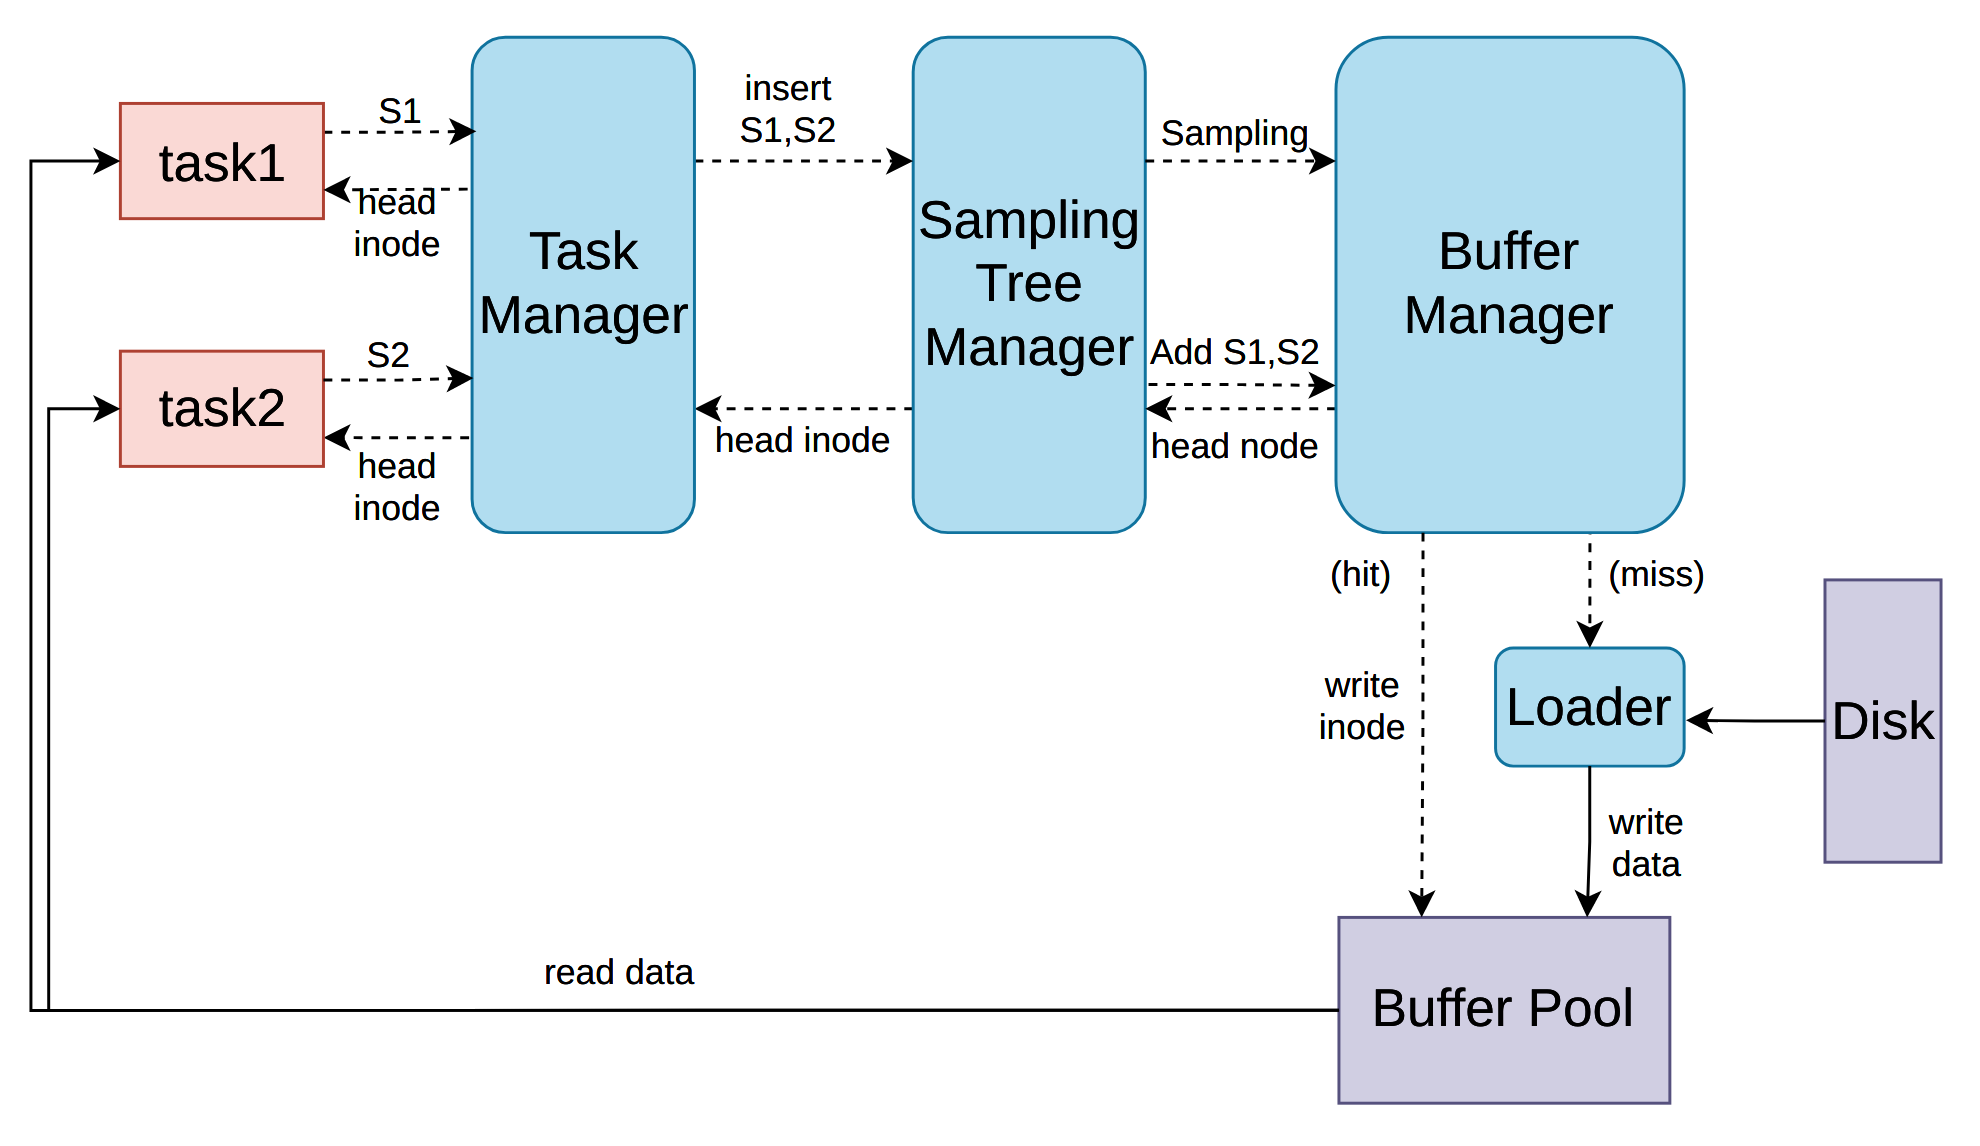
\includegraphics[width=12cm]{global_img_dir/archi.png}
\end{frame}

\begin{frame}
    \frametitle{Task Manager and Loader}
    \begin{block}{Task Manager}
        \begin{itemize}
            \item recieve task <task name, index set> and return head address
            \item send hearbeat
        \end{itemize}
    \end{block}
    \begin{block}{Loader}
        \begin{itemize}
            \item process pool
            \item read data from disk and decode them 
            \item write them in buffer pool
        \end{itemize}
    \end{block}
\end{frame}


\begin{frame}
    \frametitle{Buffer Pool: Data Structure}
    \begin{block} {data}
        \begin{itemize}
            \item There are two kinds of nodes: inode and datanode, and they are fixed size.
            \item Every task has a head inode address
        \end{itemize}
    \end{block}
    \centering
    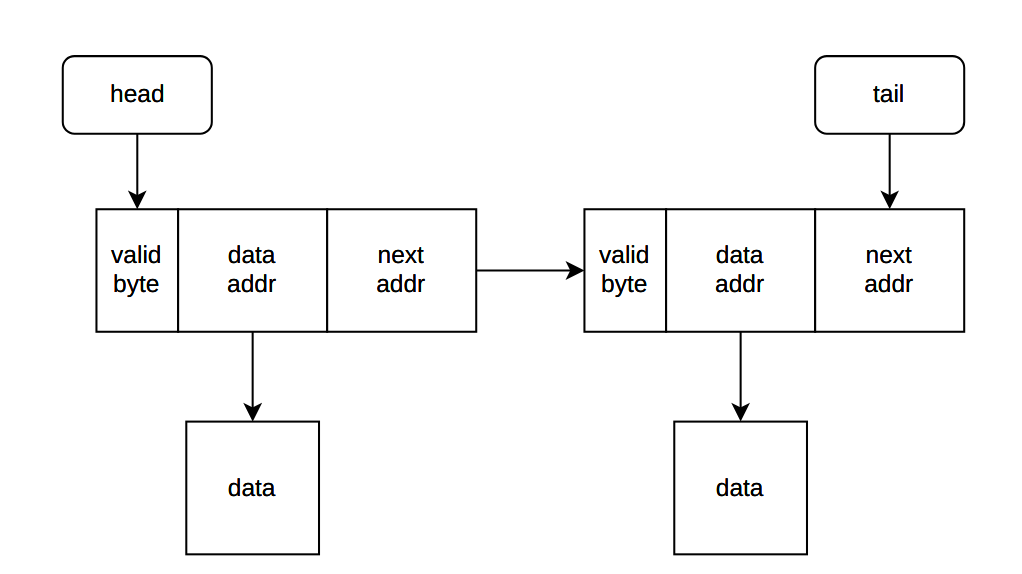
\includegraphics[width=8cm]{global_img_dir/linklist.png}
\end{frame}

\begin{frame}
    \frametitle{Buffer Pool: Valid Byte}
    \begin{block} {valid byte}
        \begin{itemize}
            \item used bit: If the used bit is equal to 1, this inode is used
            \item next bit: If the next bit is equal to 1, the next addr is valid
            \item data bit: If the data bit is equal to 1, the data addr is valid
        \end{itemize}
    \end{block}
    \centering
    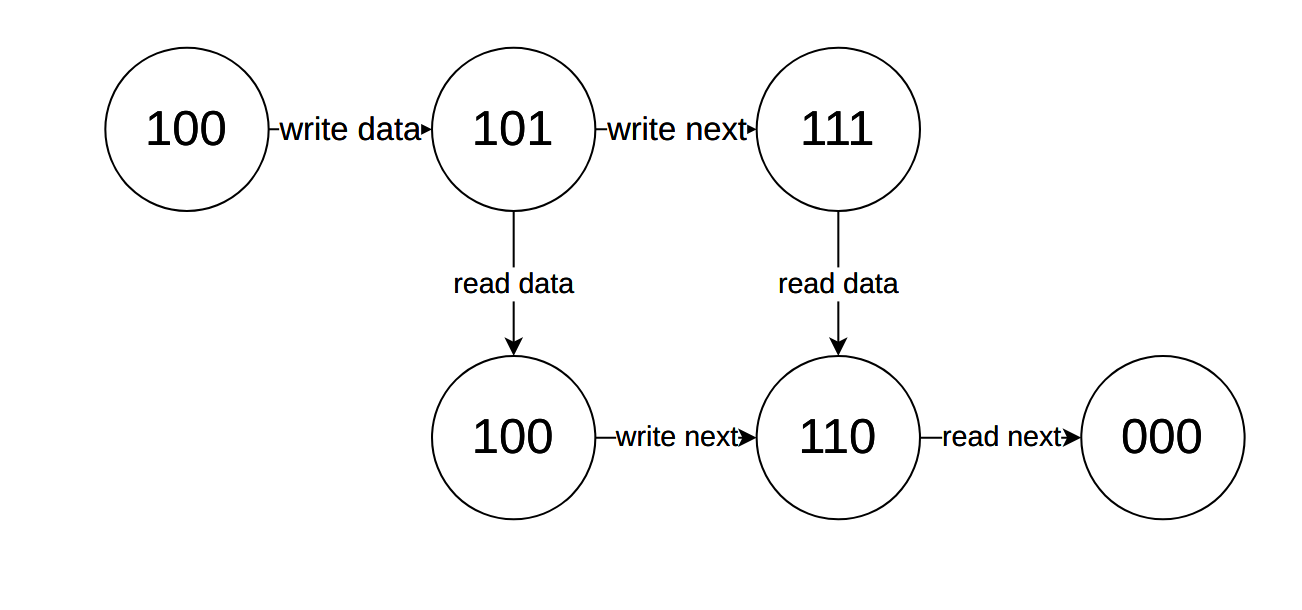
\includegraphics[width=10cm]{global_img_dir/automata.png}
\end{frame}

\begin{frame}
    \frametitle{Buffer Pool Manager}
    \begin{columns}
        \begin{column}{0.38\textwidth}
            \begin{itemize}
                \item BM is responsible for maintaining three tables
                \item BM is responsible for freeing useless nodes
            \end{itemize}
        \end{column}
        \begin{column}{0.58\textwidth}
            \begin{figure}
                \centering
                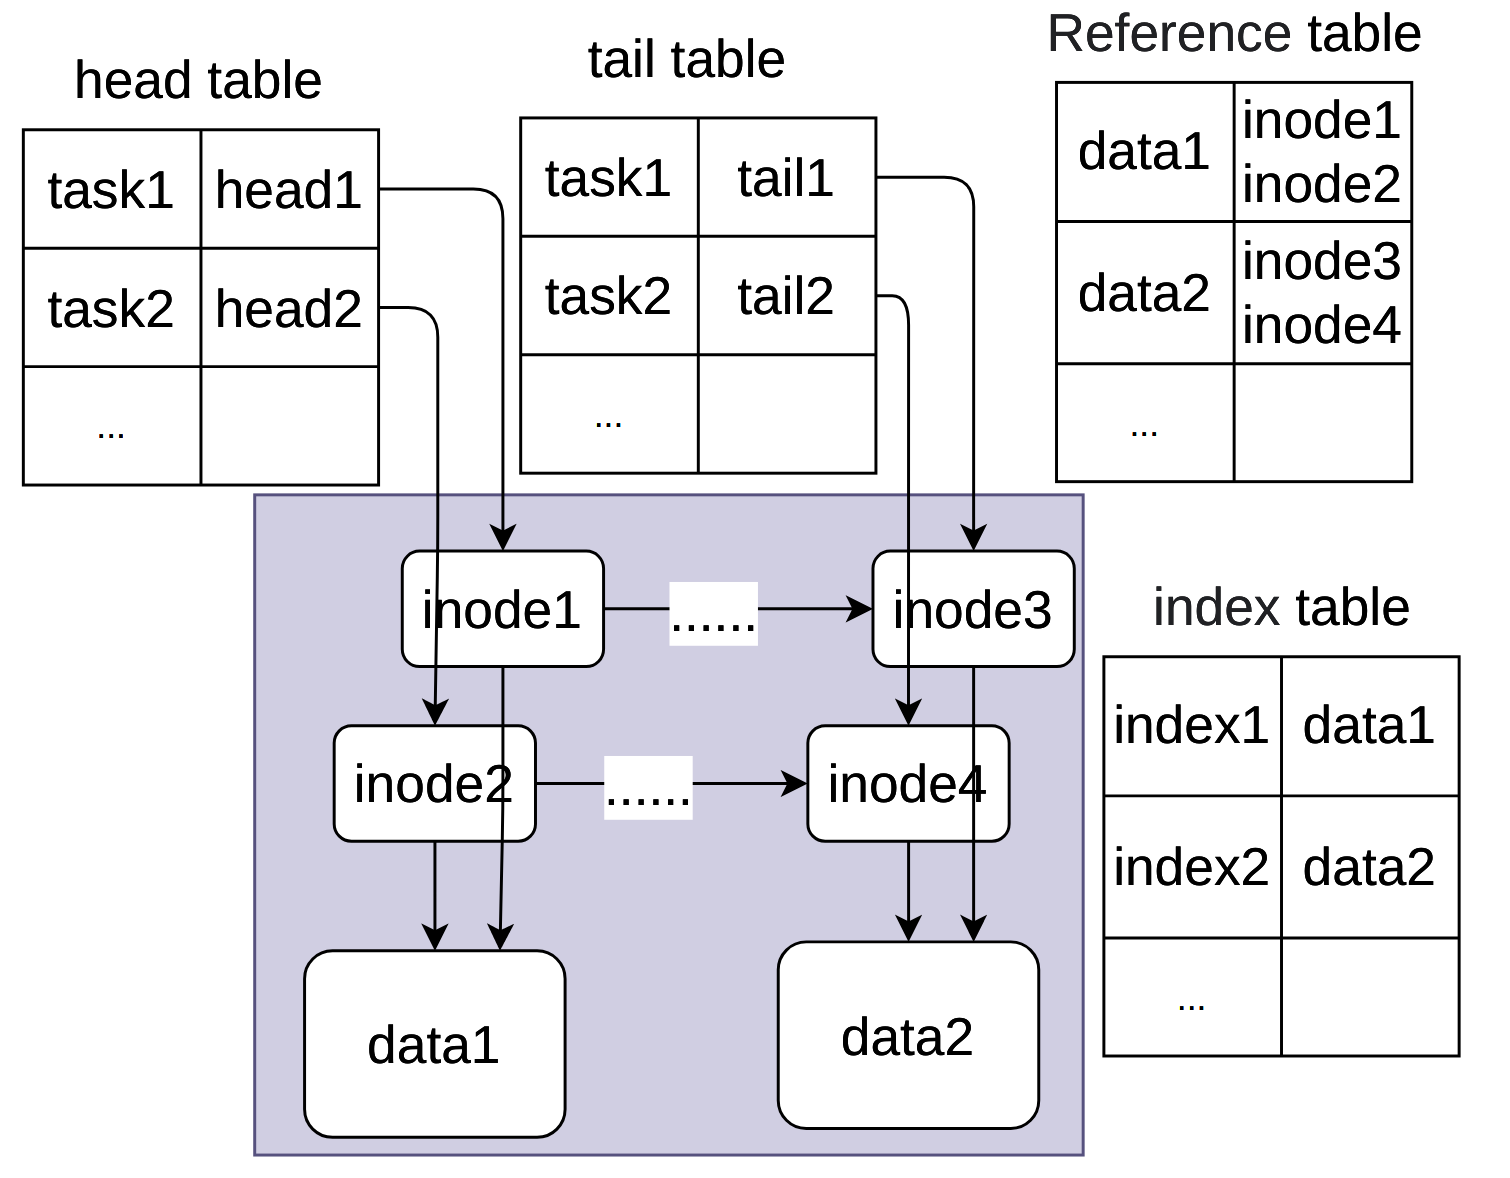
\includegraphics[width=7cm]{global_img_dir/bm.png}
                \caption{Sampling Tree}
            \end{figure}
        \end{column}
    \end{columns}
\end{frame}

\begin{frame}
    \frametitle{which data shound be free}
    \begin{block} {Expection diff}
        The difference between \\
        the number of times data has been quoted and \\
        the number of times data should be quoted
    \end{block}
    \begin{block} {Example}
        S1 = {1, 2, 3} , S2 = {1, 2} \\
        The Sampling result is {S1: 3, S2: 2} \\
        $ExpectionDiff(3) = 1-1 = 0$, \\
        $ExpectionDiff(2) = 2-1 = 1$ \\
    \end{block}
    \begin{block} {Answer}
        Choose the smallest Expection diff
    \end{block}
\end{frame}

\section{Experiment}
\begin{frame}
    \frametitle{Hit rate Experiment}
    \begin{block}{Assumption}
        There are two sets: $S_1, S_2$, and their length is $n_1, n_2$ \\
        The intersection set of them is $S_i$, whose length is $n_i$ \\
        $hitrate= \frac{hit}{n_i}$ \\
        $bufferSize = k$, which means that the buffer can have k datanode, and we ignore the size of the inode
    \end{block}
\end{frame}

\begin{frame}
    \frametitle{Hit rate}
    \begin{columns}
        \begin{column}{0.48\textwidth}
            Random replacement algorithm VS ExpectionDiff replacement algorithm
        \end{column}
        \begin{column}{0.48\textwidth}
            \begin{figure}
                \centering
                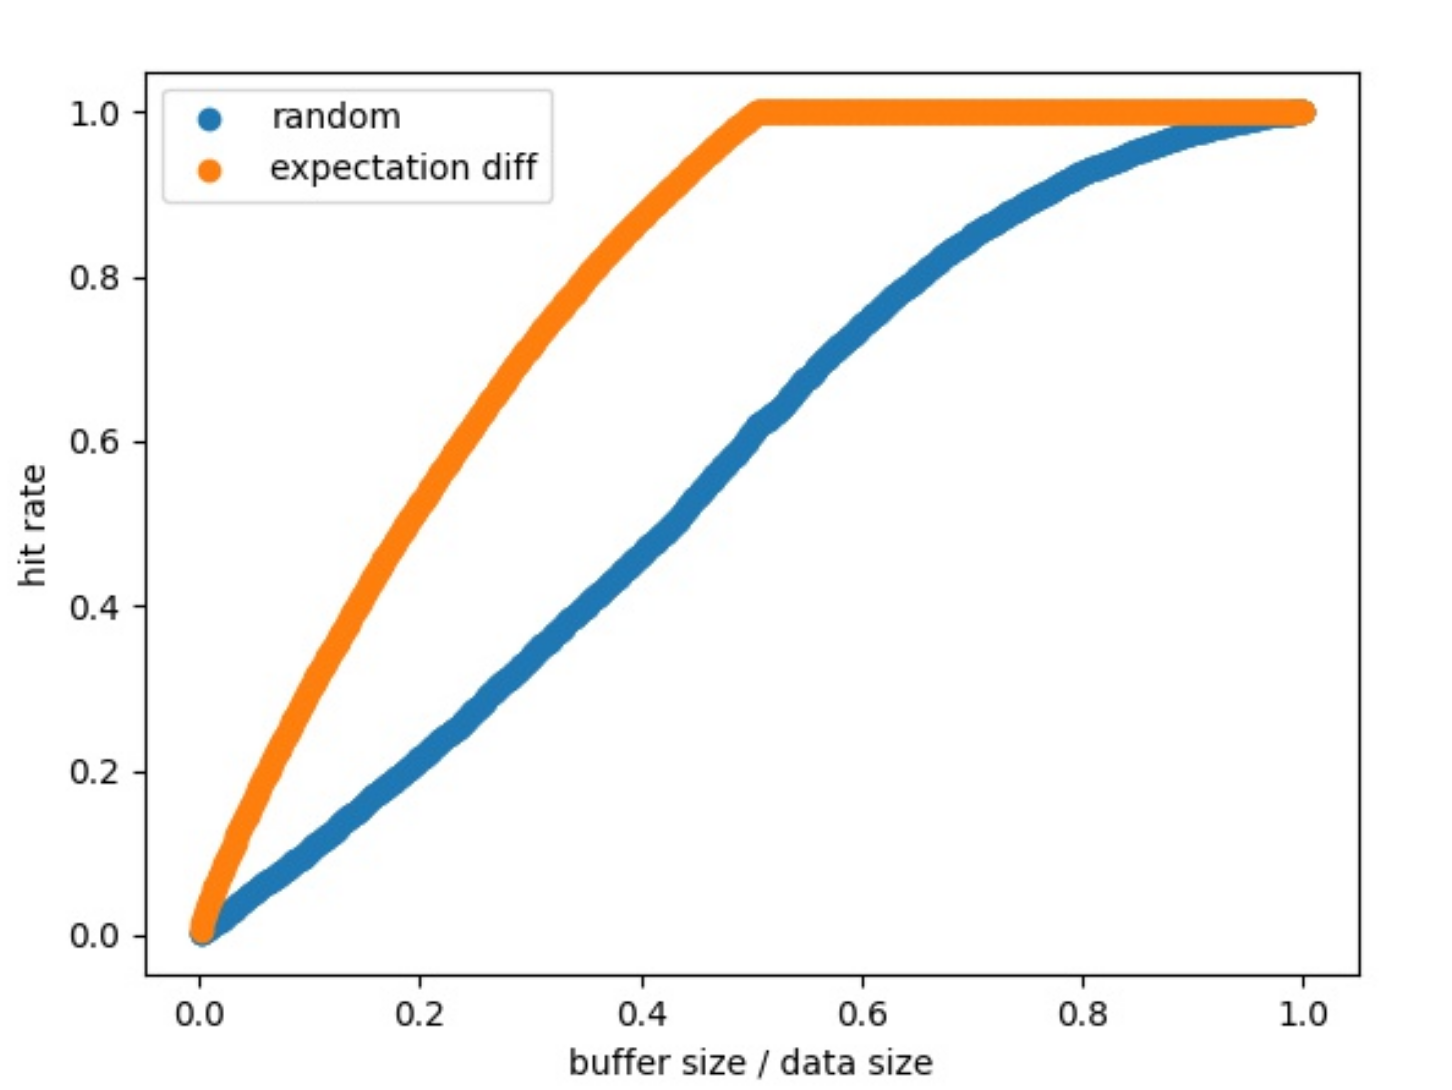
\includegraphics[width=6cm]{global_img_dir/replacement_vs.png}
                \caption{}
            \end{figure}
        \end{column}
    \end{columns}
\end{frame}

\begin{frame}
    \frametitle{Number of orphans}
    \begin{columns}
        \begin{column}{0.48\textwidth}
            $p(e_1=e_2|e_2\in S_i) = \frac{n_1}{n_2}$ \\
            Assume $p = \frac{n_1}{n_2}$
            \begin{equation}
                \begin{aligned}
                    N &= \sum_{i=0}^{n_i}{(1-\frac{n_1-i}{n_2-i})} \\
                      &\geq \sum_{i=0}^{n_1}{(1-\frac{n_1-i}{n_2-i})} \\
                      &= \sum_{i=0}^{p*n_2}{(1-\frac{p*n_2-i}{n_2-i})}\\
                      &\approx \int_{i=0}^{p*n_2}{(1-\frac{p*n_2-i}{n_2-i})}\\
                      &= n_2*(p-1)ln^{1-p}
                \end{aligned}
            \end{equation}
        \end{column}
        \begin{column}{0.48\textwidth}
            \begin{figure}
                \centering
                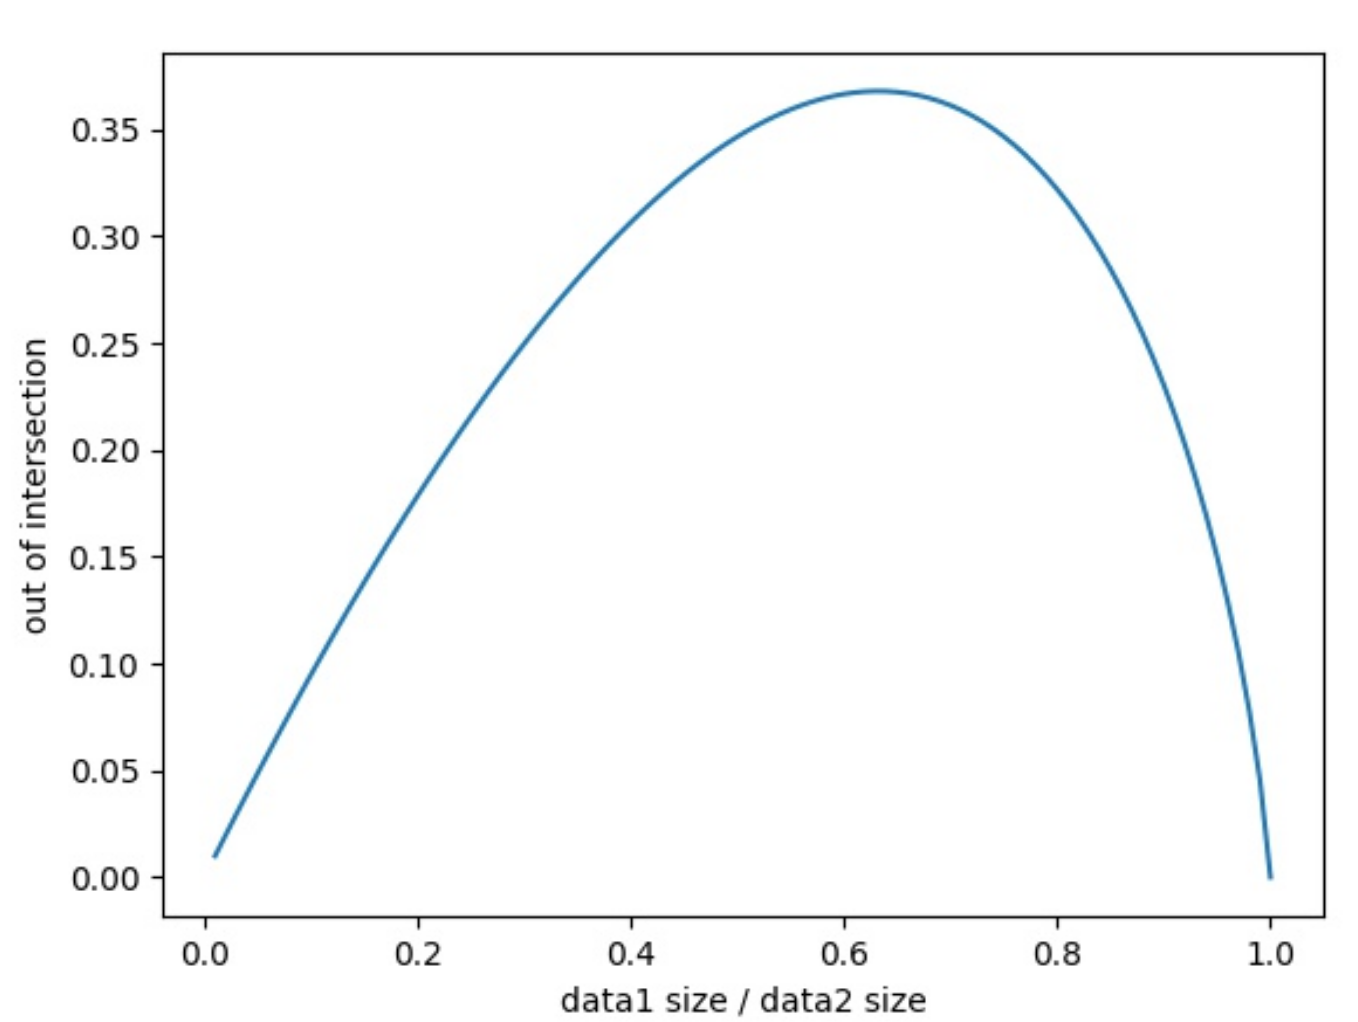
\includegraphics[width=6cm]{global_img_dir/op1.png}
                \caption{}
            \end{figure}
        \end{column}
    \end{columns}
\end{frame}


\begin{frame}
    \frametitle{Hit rate}
    \begin{columns}
        \begin{column}{0.48\textwidth}
            $buffer\_size = \frac{k}{n_2}$
        \end{column}
        \begin{column}{0.48\textwidth}
            \begin{figure}
                \centering
                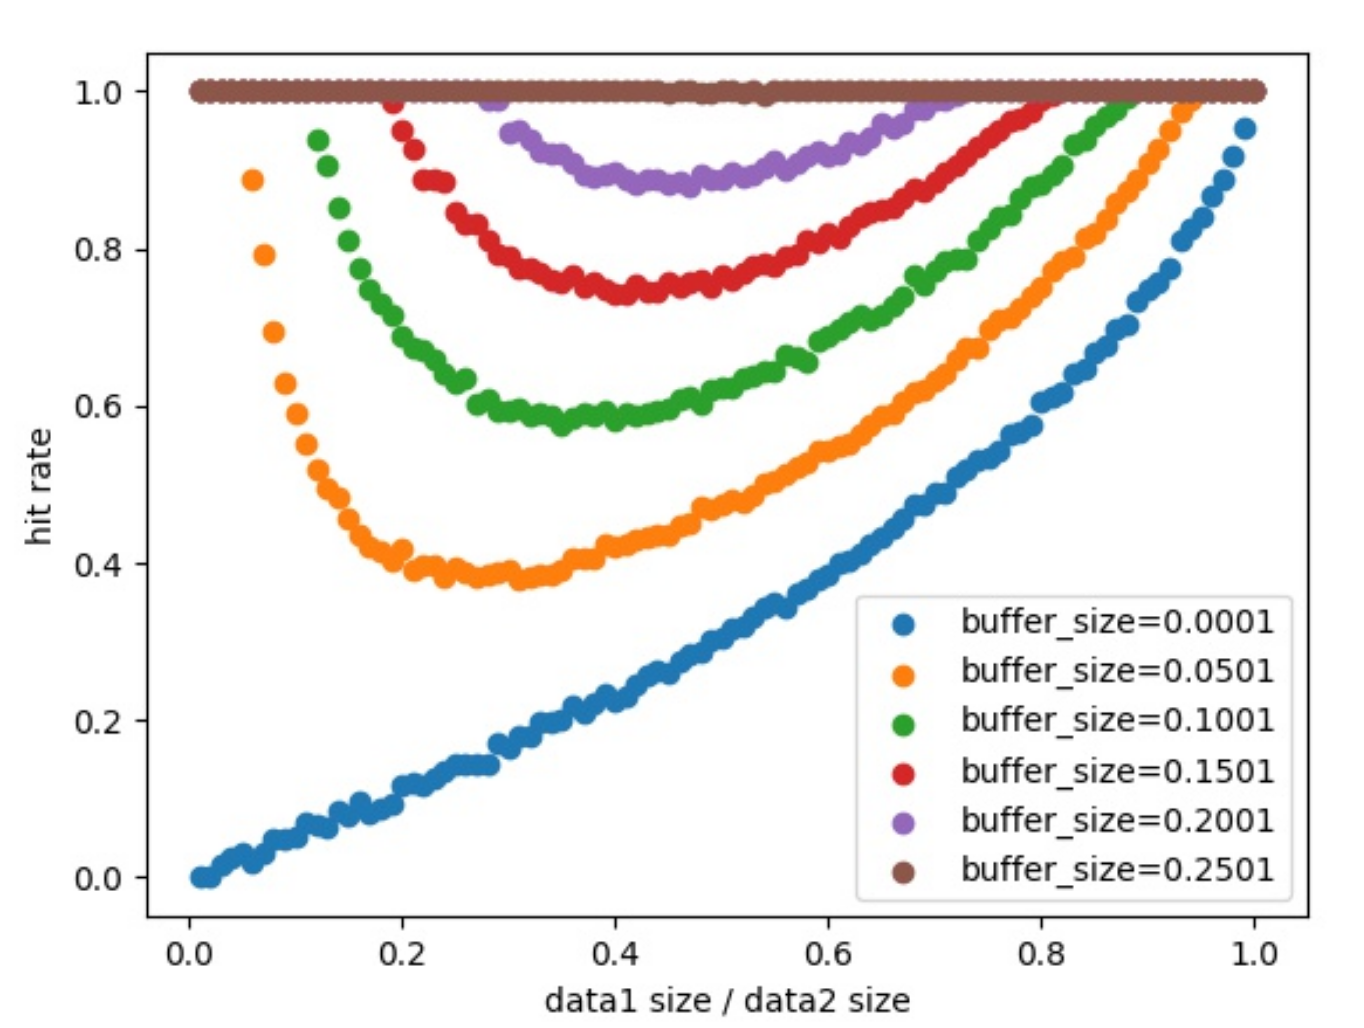
\includegraphics[width=6cm]{global_img_dir/buffer_size.png}
                \caption{}
            \end{figure}
        \end{column}
    \end{columns}
\end{frame}

\begin{frame}
    \frametitle{Time Experiment}
    \begin{figure}[htbp]
        \centering
        \begin{minipage}[t]{0.48\textwidth}
        \centering
        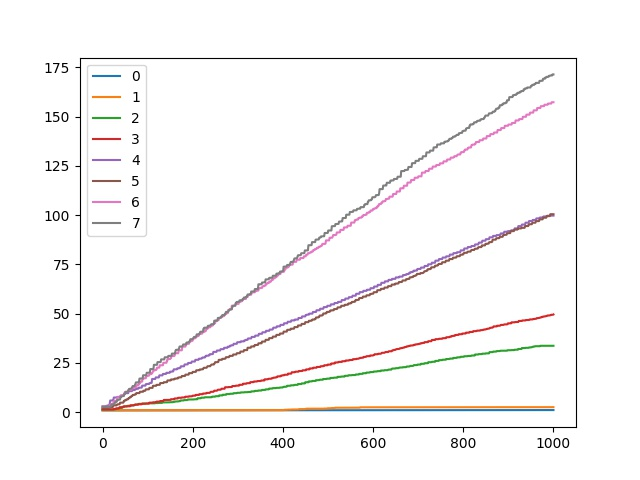
\includegraphics[width=6cm]{global_img_dir/l.jpg}
        \caption{time}
        \end{minipage}
        \begin{minipage}[t]{0.48\textwidth}
        \centering
        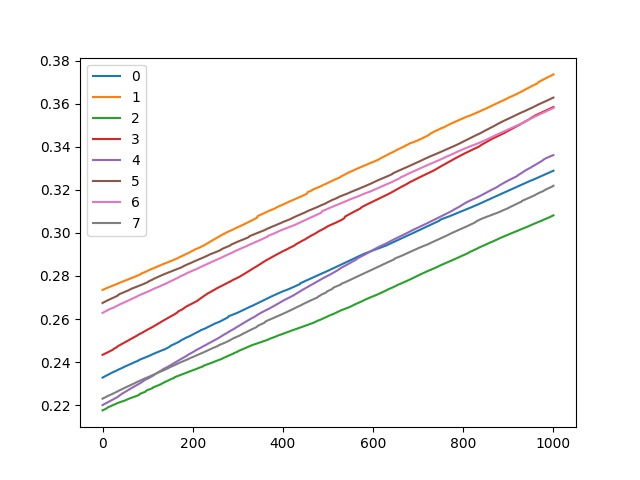
\includegraphics[width=6cm]{global_img_dir/gl.jpg}
        \caption{time with GlobalDataLoader}
        \end{minipage}
    \end{figure}
\end{frame}

\begin{frame}
    \frametitle{Correctness  Experiment}
\end{frame}

\end{document}
